\documentclass[a4paper,12pt]{report}
\usepackage[utf8]{inputenc} % To use Unicode (e.g. Turkish) characters
\usepackage[T1]{fontenc}
\renewcommand{\labelenumi}{(\roman{enumi})}
\usepackage{amsmath, amsthm, amssymb}
\usepackage{cite}
\PassOptionsToPackage{hyphens}{url}
\usepackage{url}
\Urlmuskip=0mu plus 1mu\relax
\usepackage{graphicx}
\usepackage{longtable}
\graphicspath{{figures/}}
\usepackage{booktabs}
\usepackage[protrusion=true,expansion=false]{microtype}
\usepackage{tikz}
\usetikzlibrary{shapes.geometric, arrows.meta, positioning, fit, calc, decorations.markings, backgrounds}
\usepackage{float}

\begin{document}

% Title Page
\title{CMPE 492 Final Project Report \\ VeriFi: A Reputation-Based Platform for Verifiable Financial Predictions}
\author{
Arda Saygan \\
Abdurrahman Arslan \\
Volkan Bora Seki \\
Yusuf An\i{}l Yaz\i{}c\i{} \\ \\
Advisor: \\
H\"{u}seyin Birkan Y\i{}lmaz
}
\date{}
\maketitle{}
\pagenumbering{roman}
\tableofcontents

% ─────────────────────────────────────────────────────────────────────────────
\chapter{INTRODUCTION}
\pagenumbering{arabic}

\section{Broad Impact}

The financial media landscape is plagued by unverifiable claims. Influencers, analysts, and self-proclaimed experts routinely make bold financial predictions on social media with no accountability mechanism. When predictions prove correct they are amplified; when wrong, they are quietly deleted or ignored. This asymmetry erodes public trust and enables misinformation to thrive in financial discourse.

Consider a concrete example. A popular financial influencer on Twitter (X) posts: ``Bitcoin will crash 50\% by next Friday --- sell everything now.'' Thousands of followers see the post and some act on it. When Bitcoin instead rises sharply, the influencer quietly deletes the tweet and later claims he never made such a prediction. A retail investor who lost money following the advice has no recourse: the tweet is gone, there is no proof it ever existed, and the influencer's public track record remains unblemished. On existing platforms this pattern repeats daily, because there is no technical mechanism to hold predictors accountable after deletion. The influencer's reputation is built entirely on selectively showcasing correct calls while erasing incorrect ones --- a survivorship bias that misleads followers at scale.

Now imagine the same scenario on VeriFi. When the influencer posts his prediction, the platform separates the social commentary from the structured financial claim --- ``Bitcoin, Bearish, 50\%, by next Friday'' --- and cryptographically signs the claim with the influencer's private key. A skeptical follower clicks \textit{Save Proof} and downloads the signed claim to their local device. When the prediction fails and the influencer deletes the post, the social text disappears (respecting the right to erasure), but the mathematical proof persists. The follower uploads the saved proof to VeriFi's public verification page, the system confirms the cryptographic signature matches the influencer's wallet, and the failed prediction is permanently recorded in the influencer's Truth Score. Deletion does not equal deniability.

VeriFi addresses this problem by building a social media platform where every financial prediction is cryptographically signed at the time of posting. Because the signature is generated from the author's private key and bound to the claim content, a prediction cannot be retroactively modified or plausibly denied --- even after the original post is deleted. This property, \textit{non-repudiation}, is the core differentiator of VeriFi compared to existing financial social platforms.

The platform benefits several stakeholder groups. Retail investors gain access to a transparent, tamper-proof track record of financial influencers, enabling more informed decisions about whose predictions to follow. Skilled predictors accumulate a credible, verifiable reputation that serves as a professional credential. Researchers and journalists studying financial misinformation gain a public dataset of signed, timestamped predictions with resolution outcomes.

At a societal level, VeriFi promotes financial literacy by shifting discourse toward verifiable, quantified claims and away from vague, unfalsifiable commentary. By making prediction accuracy publicly auditable, the platform creates an economic incentive for quality analysis and a natural disincentive for low-effort, clickbait content.

\section{Ethical Considerations}

Several ethical dimensions require careful attention in the design and operation of VeriFi.

\textbf{Not investment advice.} VeriFi is a reputation-tracking platform, not a financial advisory service. All content is user-generated and not endorsed by the platform operators. The platform displays a prominent disclaimer that no content constitutes investment advice, in compliance with applicable financial regulations.

\textbf{Privacy and data protection.} VeriFi deliberately avoids collecting personally identifiable information (PII). Users are identified solely by their Ethereum wallet address, a pseudonymous identifier derived from a cryptographic key pair. No names, email addresses, phone numbers, or other PII are stored. Post text is deletable by the user to accommodate GDPR and KVKK (Turkish Personal Data Protection Law) rights to erasure. However, the structured claim payload --- the financially verifiable component of a prediction --- persists even after post deletion. This design reflects the principle that while personal commentary may be retracted, quantified public financial claims carry a different epistemic status analogous to a published prediction.

\textbf{Automated extraction limitations.} The claim extraction feature assists users in structuring natural-language posts into verifiable claims. The production system uses a deterministic, rule-based extraction engine rather than an opaque model, and is designed so that the extractor serves as an assistant, not a decision-maker: every extracted claim is presented to the user for explicit confirmation, editing, or rejection before publication. The extractor never publishes claims autonomously. The system also flags when a prediction lacks a measurable target or timeframe, prompting the user to provide those fields rather than inferring them, in order to maintain verifiability.

\textbf{Sybil resistance.} A reputation system is only as trustworthy as its identity layer. By anchoring identity to a cryptographic key pair rather than a platform-controlled account, VeriFi ensures that identity manipulation requires actual cryptographic key control. The challenge-response authentication scheme prevents replay attacks. Planned features such as stake-weighted voting for soft claims further raise the economic cost of Sybil attacks.

\textbf{Fairness in resolution.} Claim resolution is performed automatically by an oracle engine that compares the predicted price movement against historical OHLC (open--high--low--close) market data fetched from multiple independent providers. Every resolution emits an immutable \texttt{HardClaimEvent} audit record containing the price data used, so resolution decisions are reproducible and auditable. Resolved claim status cannot revert, and manual resolution by a whitelisted admin address remains available only as a fallback when all data providers fail.

% ─────────────────────────────────────────────────────────────────────────────
\chapter{PROJECT DEFINITION AND PLANNING}

\section{Project Definition}

\subsection{Motivation and Problem Statement}

The financial social media landscape lacks any mechanism to hold prediction-makers accountable after the fact. Influencers, analysts, and self-styled experts publish bold financial claims to audiences of millions, yet face no structural consequences when those predictions prove incorrect. Posts can be deleted, edited, or quietly abandoned without trace, leaving followers with no verifiable record of the claims that shaped their decisions. The asymmetry between making predictions and bearing responsibility for them has created a structural trust deficit in financial discourse online.

A widely documented example illustrates the scale of this problem. In early 2022, Do Kwon, co-founder of Terraform Labs and a prominent figure in cryptocurrency social media, publicly and repeatedly declared on Twitter that the Terra ecosystem and its algorithmic stablecoin UST were fundamentally sound and that critics raising concerns about the mechanism were simply wrong --- famously responding to a sceptical economist with ``I don't debate the poor on Twitter'' \cite{quiroz2022kwon}. In May 2022, UST lost its dollar peg, triggering a cascade that caused the LUNA token to lose over 99\% of its value within 72 hours and erasing an estimated \$40 billion in market capitalisation \cite{liu2023anatomy}. The U.S. Securities and Exchange Commission subsequently charged Do Kwon and Terraform Labs with defrauding investors, and Do Kwon was sentenced in December 2025 for orchestrating what prosecutors described as a \$40 billion fraud \cite{sec2023kwon, doj2025kwon}. In the days immediately following the collapse, promotional content published by thousands of influencers who had recommended LUNA as a high-yield, low-risk asset --- along with dismissive responses directed at earlier critics --- disappeared from social media feeds. Without archived evidence, retail investors who had acted on those now-deleted recommendations were left with no verifiable record of the specific claims that had influenced their decisions and no means to establish accountability.

This is not an isolated event. The pattern of making confident financial predictions and deleting or disowning them when outcomes do not materialise recurs continuously across stock market commentary, cryptocurrency promotion, and macroeconomic forecasting. Social media platforms provide no native tooling to preserve a signed record of a published prediction. Posts can be removed without trace, and influencer profiles are routinely curated to surface only successful calls while burying failed ones, a form of survivorship bias that systematically misleads audiences about actual accuracy rates. The result is a financial social media environment that is structurally untrustworthy: followers cannot distinguish between a genuinely skilled analyst and one who simply deleted their way to a clean track record.

VeriFi proposes a technical solution to this problem. By cryptographically signing every financial prediction at the moment of publication and anchoring a public Truth Score to tamper-evident claim records, the platform makes it impossible to rewrite a predictor's history retroactively. Deletion of a post removes the social commentary but preserves the cryptographic proof, so any third party who holds a copy of the signed proof package can independently verify that a specific prediction was made, by a specific account, at a specific time. Financial credibility on VeriFi is earned through demonstrated accuracy rather than selective memory.

\subsection{System Overview}

VeriFi is a web-based social media platform for verifiable financial predictions. The central concept is the \textit{Hard Claim}: a quantified, time-bounded financial prediction with the structured fields \texttt{\{asset,\allowbreak{} direction,\allowbreak{} percentage,\allowbreak{} until\}}. Hard claims are cryptographically signed by their author at publication time. When the deadline passes, each claim is resolved as confirmed or rejected by an automated oracle engine that compares the actual asset price movement (from historical OHLC market data) against the prediction; manual resolution by an administrator exists only as a fallback.

\begin{sloppypar}
Beyond hard claims, the final system supports \textit{Positions} --- suggested trades with entry price, stop-loss, take-profit, and lifetime, tracked against market data through a full lifecycle (\texttt{pending} $\rightarrow$ \texttt{active} $\rightarrow$ \texttt{confirmed}/\texttt{rejected}/\texttt{expired}) --- and \textit{Channels}, focused sub-communities with membership roles and posting permissions.
\end{sloppypar}

Each user accumulates a \textit{Reputation Score} (\texttt{rep}), a global reputation metric earned and lost through a claim-bound prediction market: every hard claim opens a constant-product (CPMM) \textit{Reputation Market} where other users stake a fixed amount of rep on YES or NO. When the claim resolves, winning stakers receive their locked payout. The score is publicly visible, non-editable, and tamper-evident because it is anchored to cryptographically signed claim records and an auditable stake ledger.

Authentication is passwordless and wallet-based. Users either generate a native VeriFi wallet (12-word BIP39 mnemonic \cite{bip39}, secp256k1 key derivation via BIP32 \cite{bip32}, private key stored encrypted in browser \texttt{localStorage}) or connect an existing MetaMask wallet. Login uses an EIP-191 personal\_sign challenge-response flow \cite{eip191}: the server issues a single-use nonce, the client signs it with the private key, and the server recovers the signing address for verification. No password is ever stored or transmitted.

The platform is built as a monorepo with a Django REST Framework backend (deployed on Render) and a Vite/React/TypeScript frontend (deployed on Vercel). The database is SQLite in development and PostgreSQL in production.

\textbf{Delivered (v1, final):}
\begin{itemize}
    \item Wallet-based authentication (native BIP39 wallet, MetaMask, and Privy social login with Google)
    \item Hard claim creation with mandatory EIP-191 signing, feed, and user profiles
    \item Claim lifecycle management (\texttt{undetermined} $\rightarrow$ \texttt{confirmed} / \texttt{rejected})
    \item Automated oracle-based claim resolution against multi-provider OHLC market data, with full event logging and price charts
    \item Positions (suggested trades with entry, stop-loss, take-profit, and lifetime) resolved against market data
    \item Reputation Market: CPMM-based YES/NO staking on every claim with a daily energy allowance
    \item Rule-based claim extraction from free-form post text (English and Turkish)
    \item Cryptographic proof generation, download, and standalone verification page (no login required)
    \item Social layer: follows, likes, nested comments, notifications, channels, search, and asset catalog (crypto, NASDAQ, BIST, forex, commodities)
\end{itemize}

\textbf{Out of scope (v1):}
\begin{itemize}
    \item LLM-based claim extraction in production (researched and benchmarked; production uses the deterministic rule-based engine)
    \item Domain-specific reputation scores
    \item Monetization and subscription tiers
    \item Native mobile applications (the web UI is responsive)
    \item Blockchain anchoring / on-chain timestamping
\end{itemize}

\section{Project Planning}

\subsection{Project Time and Resource Estimation}

The project follows a milestone-driven development schedule aligned with the course calendar. Four milestones and a final senior presentation have been defined.

\begin{table}[thbp]
\vskip\baselineskip
\caption[Project Milestones]{Project milestones and their key deliverables.}
\begin{center}
\begin{tabular}{|c|l|p{7.5cm}|}
\hline
\textbf{Milestone} & \textbf{Date} & \textbf{Deliverables} \\\hline
M1 & March 8, 2026   & Authentication and identity: native wallet (BIP39/secp256k1), MetaMask integration, challenge-response JWT login, unified login UI \\\hline
M2 & April 5, 2026   & Core social and claim pipeline: post composer, live claim extraction, claim card UI, signed proof packages, public social feed \\\hline
M3 & May 17, 2026    & Resolution, reputation and verification: oracle integration (CoinGecko, Yahoo Finance), Truth Score, proof verifier page, feed filtering by asset \\\hline
Final & June 11, 2026 & End-to-end demo, UI/UX polish, edge case handling, performance pass, final documentation \\\hline
\end{tabular}
\label{table:milestones}
\end{center}
\end{table}

The team consists of four members, each contributing across frontend and backend work. External resource dependencies include financial data APIs (Binance, KuCoin, Kraken, CoinGecko, Yahoo Finance, Twelve Data) for oracle-based resolution, and locally hosted language models (via LM Studio) for the LLM extraction research.

\subsection{Success Criteria}

The project will be considered successful if the following criteria are met by the final presentation:

\begin{itemize}
    \item A registered user can create a hard claim; the claim is cryptographically signed and stored.
    \item A visitor can browse the public claim feed without registering.
    \item An expired claim can be resolved (confirmed or rejected) and the author's Truth Score is updated accordingly.
    \item Any third party can download a proof file and verify it on the standalone proof verification page without logging in.
    \item The system correctly rejects tampered or forged proof files.
    \item The feed page loads within 2 seconds under typical usage conditions.
    \item No critical security vulnerabilities exist in the authentication or claim submission flow.
\end{itemize}

\subsection{Risk Analysis}

\begin{table}[thbp]
\vskip\baselineskip
\caption[Risk Analysis]{Identified risks, likelihood, impact, and mitigation strategies.}
\begin{center}
\begin{tabular}{|p{3.5cm}|p{2.4cm}|p{1.5cm}|p{4.2cm}|}
\hline
\textbf{Risk} & \textbf{Likelihood} & \textbf{Impact} & \textbf{Mitigation} \\\hline
Oracle API downtime or rate limiting & Medium & High & Exponential backoff retries; fallback to secondary data source; manual admin resolution as last resort \\\hline
LLM extraction quality insufficient & High & Medium & v1 ships with manual structured entry form; LLM extraction is an enhancement, not a blocker \\\hline
Truth Score formula disputes & Medium & Medium & Formula publicly documented and fixed at v1 launch; transparent claim records allow independent verification \\\hline
Browser \texttt{localStorage} key loss & Medium & High & Mnemonic displayed and backup strongly encouraged at registration; no server-side key recovery by design \\\hline
Private key leakage from \texttt{localStorage} & Low & Critical & AES-256-GCM encryption with PBKDF2-SHA256 (100{,}000 iterations); key never transmitted to server \\\hline
GDPR / KVKK compliance & Low & High & No PII collected; post text deletable; claim payloads treated as public reputation data \\\hline
\end{tabular}
\label{table:risks}
\end{center}
\end{table}

\subsection{Team Work}

The project team consists of four members. Responsibilities are distributed as follows:

\begin{table}[thbp]
\vskip\baselineskip
\caption[Team Responsibilities]{Team member responsibilities.}
\begin{center}
\begin{tabular}{|l|p{9cm}|}
\hline
\textbf{Member} & \textbf{Primary Responsibilities} \\\hline
Arda Saygan & Backend architecture; hard claim data models and API endpoints; project repository management \\\hline
Abdurrahman Arslan & MetaMask integration; frontend PostCard and claim card UI components; requirements specification \\\hline
Volkan Bora Seki & AI/LLM infrastructure (Agno + LM Studio); multilingual claim extraction; LLM benchmark design \\\hline
Yusuf An\i{}l Yaz\i{}c\i{} & Native wallet and key management; cryptographic authentication frontend; midterm report; deployment \\\hline
\end{tabular}
\label{table:team}
\end{center}
\end{table}

The team holds weekly advisory meetings on Tuesdays (17:30--18:00) with the project advisor. Meeting notes and decisions are recorded in the project GitHub wiki. Rush weekends with concentrated development effort have been scheduled around milestone deadlines.

% ─────────────────────────────────────────────────────────────────────────────
\chapter{RELATED WORK}

The problem of tracking and verifying financial predictions has been approached from several directions in both industry and academia.

\textbf{Prediction Markets.} Prediction markets are exchange-traded platforms where users buy and sell contracts on future events, with prices reflecting aggregate probability estimates \cite{wolfers2004}. Platforms such as Polymarket and PredictIt allow users to stake real money on event outcomes, providing strong accountability: incorrect predictions result in direct financial loss. While effective for accountability, these systems are regulated as financial instruments in many jurisdictions and do not support the social media dynamics --- posts, feeds, followers, profiles --- that VeriFi targets. Augur \cite{augur2019} extends the model to a decentralised, blockchain-based architecture, but requires on-chain interaction and cryptocurrency holdings, creating a high barrier for casual users.

\textbf{Social Trading Platforms.} eToro and similar platforms allow users to publish and copy investment portfolios, providing a form of reputation tracking based on actual trade performance. However, these platforms require linking real brokerage accounts, making them inaccessible to users who wish to share predictions without executing trades. StockTwits provides a Twitter-like social layer for financial commentary but lacks any systematic verification or scoring mechanism: predictions and outcomes are not tracked.

\textbf{Reputation Systems.} Reputation systems in online communities, such as Stack Overflow's karma system or academic citation indices, have been studied extensively \cite{josang2007}. A key finding is that reputation scores are only as trustworthy as the underlying identity system and the non-repudiability of the actions they measure. VeriFi applies this insight to financial predictions by anchoring reputation to cryptographic identity and signed claim records.

\textbf{Cryptographic Non-Repudiation.} The use of digital signatures for non-repudiation of electronic documents is well established \cite{johnson2001}. Ethereum's EIP-191 personal\_sign standard \cite{eip191} extends this to wallet-based signatures, which VeriFi uses as the foundation of its proof system. The key contribution of VeriFi is applying this mechanism to social media content --- specifically financial predictions --- so that deletion or denial of a claim becomes cryptographically impossible for anyone who has saved the signed proof.

\textbf{LLM-Assisted Structured Extraction.} Recent work on large language model-based information extraction has demonstrated strong performance on converting natural language into structured records \cite{wei2022}. VeriFi uses an LLM (via the Agno framework with a locally hosted model) to assist users in extracting structured \texttt{\{asset, direction, percentage, timeframe\}} tuples from free-form text. A critical design constraint, derived from team discussions, is that the LLM must not infer missing fields --- especially timeframes --- but must prompt the user to supply them explicitly, preserving the verifiability of every published claim.

% ─────────────────────────────────────────────────────────────────────────────
\chapter{METHODOLOGY}

VeriFi is built as a monorepo web application with clearly separated frontend and backend layers.

\begin{sloppypar}
\textbf{Backend.} The backend is a REST API built with Django 6 and Django REST Framework (DRF). Authentication uses \texttt{djangorestframework-simplejwt} for JWT issuance and validation, and the \texttt{eth-account} library for Ethereum signature verification. The backend is stateless: no server-side sessions are maintained. All authentication state is encoded in the JWT token. The database is SQLite in development and PostgreSQL in production (Render).
\end{sloppypar}

\textbf{Frontend.} The frontend is a React 19 + TypeScript single-page application (SPA) built with Vite 7. UI components use Tailwind CSS v4 and the shadcn/ui component library. Cryptographic operations (BIP39 mnemonic generation, BIP32 key derivation, secp256k1 signing, AES-256-GCM key encryption) are performed entirely client-side using \texttt{@scure/bip39}, \texttt{@scure/bip32}, \texttt{@noble/secp256k1}, and \texttt{@noble/hashes} --- pure TypeScript implementations with no native dependencies. The frontend is deployed on Vercel.

\textbf{Authentication.} The authentication system is passwordless and wallet-based. Two wallet modes are supported: (1) a native VeriFi wallet based on BIP39 mnemonic generation and BIP32/BIP44 key derivation, with the private key stored AES-256-GCM encrypted in browser \texttt{localStorage}; and (2) MetaMask via the EIP-1193 browser extension API. Both modes use an identical EIP-191 personal\_sign challenge-response flow for login, described in full in Section~\ref{sec:auth_design}.

\textbf{Claim Signing.} Every hard claim is cryptographically signed with the author's secp256k1 private key at creation time. The signature covers a canonical JSON serialisation of the claim payload: \texttt{\{author\_address, asset, direction, percentage, until, server\_timestamp\}}. This produces a proof bundle that allows any third party to verify --- using only the standard Ethereum public-key infrastructure --- that a specific user made a specific prediction at a specific time.

\textbf{Claim Extraction.} The system includes a claim extraction endpoint (\texttt{POST /api/posts/extract-claims/}) backed by a deterministic, rule-based extraction engine with no AI dependency at runtime. The engine combines an asset whitelist with alias mapping (e.g.\ ``Bitcoin'', ``BTC'', ``bitcoin dolar''), fuzzy matching, and a set of regular-expression patterns for directions, percentage and absolute price targets, and relative or absolute timeframes, in both English and Turkish. As the user types a post, the frontend calls the endpoint with debouncing and displays detected claims live; each extracted claim is presented as a Claim Card for explicit confirmation, editing, or rejection before publication. An LLM-based extractor (Agno framework with locally hosted models) was researched and benchmarked in parallel (Section~\ref{sec:ai_engine}); the deterministic engine was chosen for production because it is reproducible, fast, free to operate, and cannot hallucinate fields.

\textbf{Oracle-Based Resolution.} Claim resolution is automated by a backend resolution engine. At claim creation, the reference (entry) price is captured from an intraday quote and stored on the claim. Upon expiry --- or on demand for an early hit --- the engine fetches historical OHLC candles for the claim window from a fallback chain of independent providers (Binance, KuCoin, and Kraken for cryptocurrency; Yahoo Finance and Twelve Data for equities, forex, and commodities; CoinGecko as an additional crypto fallback) and evaluates whether the asset moved at least \texttt{percentage}\% in the predicted \texttt{direction} at any point between creation and the \texttt{until} date. Evaluating the peak (or trough) over the whole window, rather than only the closing price at the deadline, means a prediction that was demonstrably correct mid-window cannot be retroactively falsified by a later reversal. Candles before claim creation are excluded so that pre-entry moves on the creation day cannot confirm a claim. Every resolution writes a \texttt{HardClaimEvent} audit record, fetched OHLC rows are cached in the database, resolution is idempotent, and a resolved status cannot revert.

\textbf{Reputation Market.} Each user's Reputation Score (\texttt{rep}) is earned and lost through a constant-product market maker (CPMM) prediction market attached to every hard claim --- the same mechanism used by Polymarket-style prediction markets \cite{wolfers2004}. The claim author funds the initial market depth with a creator stake (10--100 rep) on the side of their own claim, and pays a small listing fee that is burned. Other users stake a fixed 10 rep on YES or NO; the CPMM prices each purchase, and the buyer's payout is locked at purchase time. When the oracle resolves the claim, winning shares each pay out 1 rep, the creator additionally receives 5\% of the losing side's net pool, and a 5\% fee on every trade is burned to control rep inflation. Markets with too little genuine disagreement (fewer than 3 distinct dissenters or 5 total stakers) refund all stakes, closing the trivial-claim farming loophole. A separate daily \textit{energy} allowance (3 per day, lazily granted) limits how many stakes and claims each user can place, keeping the leaderboard competitive for new users. This design --- internally ``Model G'' --- was selected through an extensive simulation study described in Section~\ref{sec:rep_simulation}.

% ─────────────────────────────────────────────────────────────────────────────
\chapter{REQUIREMENTS SPECIFICATION}

\section{Stakeholders and User Personas}

\begin{table}[thbp]
\vskip\baselineskip
\caption[Stakeholders]{Stakeholders and their primary interactions with the system.}
\begin{center}
\begin{tabular}{|l|p{4.5cm}|p{5.5cm}|}
\hline
\textbf{Persona} & \textbf{Description} & \textbf{Primary Actions} \\\hline
Predictor & Registered user who makes financial claims & Register, login, create claims, view profile \\\hline
Visitor & Unauthenticated user browsing the platform & View feed, view profiles, verify proofs \\\hline
Admin & Whitelisted wallet address (Ethereum) & Manually resolve claim status via API \\\hline
Proof Verifier & Anyone with a downloaded proof file & Upload proof to the standalone verification page \\\hline
\end{tabular}
\label{table:stakeholders}
\end{center}
\end{table}

\section{Functional Requirements}

\subsection{Authentication}

The system provides passwordless, wallet-based login. No email or password is stored on any server. Two flows are supported: native BIP39 wallet and MetaMask.

\begin{table}[thbp]
\vskip\baselineskip
\caption[Authentication Requirements]{Authentication functional requirements.}
\begin{center}
\begin{tabular}{|l|p{11cm}|}
\hline
\textbf{ID} & \textbf{Requirement} \\\hline
AUTH-01 & The system MUST generate a 12-word BIP39 mnemonic in-browser on the client without server involvement. \\\hline
AUTH-02 & The system MUST derive a secp256k1 key pair from the mnemonic using BIP32 path \texttt{m/44'/60'/0'/0/0}. \\\hline
AUTH-03 & The Ethereum address MUST be derived as the last 20 bytes of \texttt{keccak256(uncompressedPublicKey[1:])}, prefixed with \texttt{0x}. \\\hline
AUTH-04 & The user MUST explicitly acknowledge that they have saved their mnemonic before registration proceeds. \\\hline
AUTH-05 & The private key MUST be encrypted with AES-256-GCM using a PBKDF2-SHA256 derived key (100,000 iterations, random salt and IV) before being stored in \texttt{localStorage}. \\\hline
AUTH-06 & The server MUST reject duplicate wallet address registrations with HTTP 409. \\\hline
AUTH-07 & On successful registration, the server MUST return a JWT access token. \\\hline
AUTH-08 & The client MUST request a nonce via \texttt{GET /api/auth/challenge/?address=<addr>}. \\\hline
AUTH-09 & The server MUST generate a cryptographically random 256-bit nonce and store it with a 5-minute TTL. \\\hline
AUTH-10 & The client MUST sign the nonce using EIP-191 \texttt{personal\_sign} with the decrypted private key. \\\hline
AUTH-11 & The server MUST recover the signer address from the signature and reject if it does not match the claimed address. \\\hline
AUTH-12 & The nonce MUST be deleted from cache immediately after first verification attempt (single-use). \\\hline
AUTH-13 & On successful login, the server MUST return a JWT with the lowercase wallet address claim and a 7-day lifetime. \\\hline
AUTH-14 & The system MUST support MetaMask (EIP-1193 provider) as an alternative login method using the same backend endpoints. \\\hline
AUTH-15 & When MetaMask is used, VeriFi MUST NOT store or transmit the private key; signing is delegated entirely to MetaMask. \\\hline
AUTH-16 & JWTs MUST be stored in \texttt{localStorage["verifi\_jwt"]}; wallet address in \texttt{localStorage["verifi\_address"]}. \\\hline
AUTH-17 & All stateful write endpoints MUST validate the JWT and extract the \texttt{address} claim to identify the acting user. \\\hline
AUTH-18 & Logout MUST clear the JWT, address, and encrypted private key from \texttt{localStorage}. \\\hline
\end{tabular}
\label{table:auth_req}
\end{center}
\end{table}

\subsection{Hard Claim Creation}

\begin{table}[thbp]
\vskip\baselineskip
\caption[Hard Claim Requirements]{Hard claim creation functional requirements.}
\begin{center}
\begin{tabular}{|l|p{11cm}|}
\hline
\textbf{ID} & \textbf{Requirement} \\\hline
CLM-01 & A hard claim MUST contain all four fields: \texttt{asset}, \texttt{direction} (\texttt{Bullish}/\texttt{Bearish}), \texttt{percentage} (float, 0--100), \texttt{until} (future date). \\\hline
CLM-02 & The \texttt{until} date MUST be strictly in the future at time of submission; the backend MUST enforce this constraint. \\\hline
CLM-03 & The \texttt{percentage} field MUST be between 0 and 100; validated on the backend. \\\hline
CLM-04 & A hard claim MUST be linked to the authenticated user's wallet address as \texttt{author}. \\\hline
CLM-05 & The initial status of a new hard claim MUST be \texttt{undetermined}. \\\hline
CLM-06 & The \texttt{asset} field MUST reference a pre-defined \texttt{Asset} record (id, name, symbol, description) from the backend. \\\hline
CLM-07 & The \texttt{text} field contains the user's free-form natural-language description of their prediction. \\\hline
\end{tabular}
\label{table:claim_req}
\end{center}
\end{table}

\subsection{Claim Extraction}

The endpoint \texttt{POST /api/posts/extract-claims/} is served by the deterministic rule-based extraction engine described in the Methodology chapter.

\begin{table}[thbp]
\vskip\baselineskip
\caption[Claim Extraction Requirements]{Claim extraction functional requirements.}
\begin{center}
\begin{tabular}{|l|p{11cm}|}
\hline
\textbf{ID} & \textbf{Requirement} \\\hline
CLM-E01 & The extraction engine MUST extract hard claim candidates from free-form post text in English and Turkish. \\\hline
CLM-E02 & A valid extracted claim requires all four fields: \texttt{asset}, \texttt{direction}, \texttt{target\_value}, \texttt{timeframe\_iso}. \\\hline
CLM-E03 & If a required field is missing, the system MUST prompt the user to fill it in explicitly --- no inference or generic defaults. \\\hline
CLM-E04 & Each extracted claim MUST be presented as a Claim Card for user confirmation, editing, or rejection before posting. \\\hline
CLM-E05 & The extraction response schema MUST be: \texttt{\{claims: [\{asset, direction, target\_value, target\_unit, timeframe\_iso, language\}]\}}. \\\hline
CLM-E06 & The extraction engine is stateless and deterministic; each call is independent and reproducible. \\\hline
\end{tabular}
\label{table:llm_req}
\end{center}
\end{table}

\subsection{Claim Resolution}

\begin{table}[thbp]
\vskip\baselineskip
\caption[Resolution Requirements]{Claim resolution functional requirements.}
\begin{center}
\begin{tabular}{|l|p{11cm}|}
\hline
\textbf{ID} & \textbf{Requirement} \\\hline
RES-01 & A claim MUST be resolved to either \texttt{confirmed} or \texttt{rejected} after its \texttt{until} date passes. \\\hline
RES-02 & Only wallet addresses listed in \texttt{ADMIN\_ADDRESSES} (server config) MAY call the claim status update endpoint. \\\hline
RES-03 & The update endpoint MUST accept \texttt{\{"status": "confirmed"|"undetermined"|"rejected"\}} and persist the change. \\\hline
RES-04 & Automated resolution: the system MUST detect expired claims and query the oracle engine to determine the outcome from OHLC data covering the claim window. \\\hline
RES-05 & Oracle selection: Binance / KuCoin / Kraken / CoinGecko for crypto assets; Yahoo Finance / Twelve Data for traditional assets, with per-asset provider symbol mapping. \\\hline
RES-06 & Oracle failures MUST fall through a provider fallback chain; if all providers fail, status remains \texttt{undetermined} and manual admin resolution is available. \\\hline
RES-07 & Resolution results MUST be permanent and auditable; a resolved claim status MUST NOT revert. \\\hline
\end{tabular}
\label{table:resolution_req}
\end{center}
\end{table}

\subsection{Cryptographic Proofs}

Every claim and position carries a mandatory EIP-191 signature, enforced server-side; the standalone verification page is publicly accessible.

\begin{table}[thbp]
\vskip\baselineskip
\caption[Proof Requirements]{Cryptographic proof functional requirements.}
\begin{center}
\begin{tabular}{|l|p{11cm}|}
\hline
\textbf{ID} & \textbf{Requirement} \\\hline
PRF-01 & Every hard claim MUST be signed with the author's secp256k1 private key at creation time. \\\hline
PRF-02 & The proof package MUST contain: \texttt{\{claim\_payload (JSON), signature (hex), wallet\_address, server\_timestamp\}}. \\\hline
PRF-03 & Any authenticated user MUST be able to download a claim's proof as a local JSON file. \\\hline
PRF-04 & A standalone public verification page MUST allow anyone (no login required) to upload a proof JSON and verify its authenticity. \\\hline
PRF-05 & Deleting a post or deactivating an account MUST NOT invalidate a previously generated claim proof. \\\hline
PRF-06 & Proof verification MUST recover the signer address from the signature and compare it to the stored \texttt{wallet\_address}. \\\hline
\end{tabular}
\label{table:proof_req}
\end{center}
\end{table}

\subsection{Reputation Market}

\begin{table}[thbp]
\vskip\baselineskip
\caption[Reputation Market Requirements]{Reputation market functional requirements.}
\begin{center}
\begin{tabular}{|l|p{11cm}|}
\hline
\textbf{ID} & \textbf{Requirement} \\\hline
REP-01 & Each user MUST have a single global numeric Reputation Score (\texttt{rep}), starting at 200. \\\hline
REP-02 & Every hard claim MUST open a CPMM market; the creator funds it with a stake of 10--100 rep on their own side and pays a 2-rep listing fee (burned). \\\hline
REP-03 & A user MAY hold at most one stake per claim, at a fixed 10 rep; a 5\% trade fee is burned. \\\hline
REP-04 & Payouts MUST be locked at purchase time (1 rep per winning share); later trades MUST NOT change earlier buyers' payouts. \\\hline
REP-05 & On resolution, the creator MUST additionally receive 5\% of the losing side's net pool if their side wins. \\\hline
REP-06 & Markets with fewer than 3 distinct losing-side stakers or fewer than 5 total stakers MUST refund all stakes (trivial-claim protection). \\\hline
REP-07 & Each stake and each claim creation MUST cost 1 energy; users receive 3 energy per UTC day (lazily granted, starting at 4). \\\hline
REP-08 & A claim with status \texttt{undetermined} MUST NOT pay out until resolved; all stakes MUST be auditable per user and per claim. \\\hline
\end{tabular}
\label{table:truth_req}
\end{center}
\end{table}

\subsection{Feed}

\begin{table}[thbp]
\vskip\baselineskip
\caption[Feed Requirements]{Feed functional requirements.}
\begin{center}
\begin{tabular}{|l|p{11cm}|}
\hline
\textbf{ID} & \textbf{Requirement} \\\hline
FEED-01 & A public feed MUST display all hard claims sorted by creation time (descending). \\\hline
FEED-02 & Each claim card MUST show: author wallet address, asset, direction, percentage target, deadline, and status badge (\texttt{Undetermined} / \texttt{Confirmed} / \texttt{Rejected}). \\\hline
FEED-03 & The feed MUST be filterable by asset and asset category without page reload. \\\hline
FEED-04 & Feed data MUST be accessible to unauthenticated users. \\\hline
FEED-05 & The feed MUST load in under 2 seconds under normal conditions. \\\hline
\end{tabular}
\label{table:feed_req}
\end{center}
\end{table}

\subsection{User Profiles}

\begin{table}[thbp]
\vskip\baselineskip
\caption[Profile Requirements]{User profile functional requirements.}
\begin{center}
\begin{tabular}{|l|p{11cm}|}
\hline
\textbf{ID} & \textbf{Requirement} \\\hline
PRF-P01 & Every wallet address MUST have a publicly accessible profile page. \\\hline
PRF-P02 & A profile MUST display: username, wallet address, Reputation Score, and full claim, position, and post history. \\\hline
PRF-P03 & Claim history MUST include a per-claim proof download link. \\\hline
PRF-P04 & Users MUST be able to filter another user's profile by wallet address (search). \\\hline
PRF-P05 & The profile page MUST allow the authenticated owner to reveal their encrypted private key temporarily (60-second auto-hide). \\\hline
PRF-P06 & The revealed private key MUST be displayed partially obfuscated (\texttt{first8\ldots last8}) with a copy-to-clipboard option. \\\hline
\end{tabular}
\label{table:profile_req}
\end{center}
\end{table}

\section{Non-Functional Requirements}

\subsection{Security}

\begin{table}[thbp]
\vskip\baselineskip
\caption[Security NFRs]{Security non-functional requirements.}
\begin{center}
\begin{tabular}{|p{4cm}|p{8.5cm}|}
\hline
\textbf{Requirement} & \textbf{Detail} \\\hline
Private key isolation & Private key MUST never be transmitted to any server. Only the derived public address is known to the server. \\\hline
Local key encryption & Private key MUST be encrypted with AES-256-GCM + PBKDF2-SHA256 (100,000 iterations) before storage. \\\hline
Nonce replay prevention & Nonces are single-use; deleted from cache immediately after first verification attempt. TTL: 5 minutes. \\\hline
JWT security & JWT MUST be signed with \texttt{SECRET\_KEY} (environment variable in production). Lifetime: 7 days. \\\hline
CORS & \texttt{CORS\_ALLOWED\_ORIGINS} MUST be restricted to the known frontend origin; wildcard MUST NOT be used in production. \\\hline
Admin authorization & Only addresses in \texttt{ADMIN\_ADDRESSES} may call claim resolution endpoints; checked server-side on every request. \\\hline
\end{tabular}
\label{table:security_nfr}
\end{center}
\end{table}

\subsection{Privacy and GDPR / KVKK}

\begin{table}[thbp]
\vskip\baselineskip
\caption[Privacy NFRs]{Privacy and data protection non-functional requirements.}
\begin{center}
\begin{tabular}{|p{4cm}|p{8.5cm}|}
\hline
\textbf{Requirement} & \textbf{Detail} \\\hline
No PII stored & No email, phone number, real name, or other personally identifiable information is stored. \\\hline
Post text deletion & Users MUST be able to request deletion of post text (GDPR / KVKK right to erasure). \\\hline
Claim payload permanence & Signed claim payloads are mathematical accountability data and MAY persist after post text deletion. \\\hline
Pseudonymous identity & Wallet address is a pseudonymous identifier; users choose how much real-world identity to attach. \\\hline
\end{tabular}
\label{table:privacy_nfr}
\end{center}
\end{table}

\subsection{Performance and Reliability}

\begin{table}[thbp]
\vskip\baselineskip
\caption[Performance NFRs]{Performance and reliability non-functional requirements.}
\begin{center}
\begin{tabular}{|p{5cm}|p{7.5cm}|}
\hline
\textbf{Requirement} & \textbf{SLA / Detail} \\\hline
Feed initial load & $<$ 2 seconds under normal conditions \\\hline
LLM claim extraction & $<$ 10 seconds per extraction call (when implemented) \\\hline
Claim resolution job & Must run within 5 minutes of \texttt{until} date expiry \\\hline
Proof verification & $<$ 1 second (client-side computation) \\\hline
Oracle retries & Exponential backoff on oracle failure; resolution job MUST be idempotent \\\hline
Claim data durability & Claim records MUST survive post deletions and account deactivations \\\hline
\end{tabular}
\label{table:performance_nfr}
\end{center}
\end{table}

\begin{figure}[p]
\centering
\resizebox{\textwidth}{!}{%
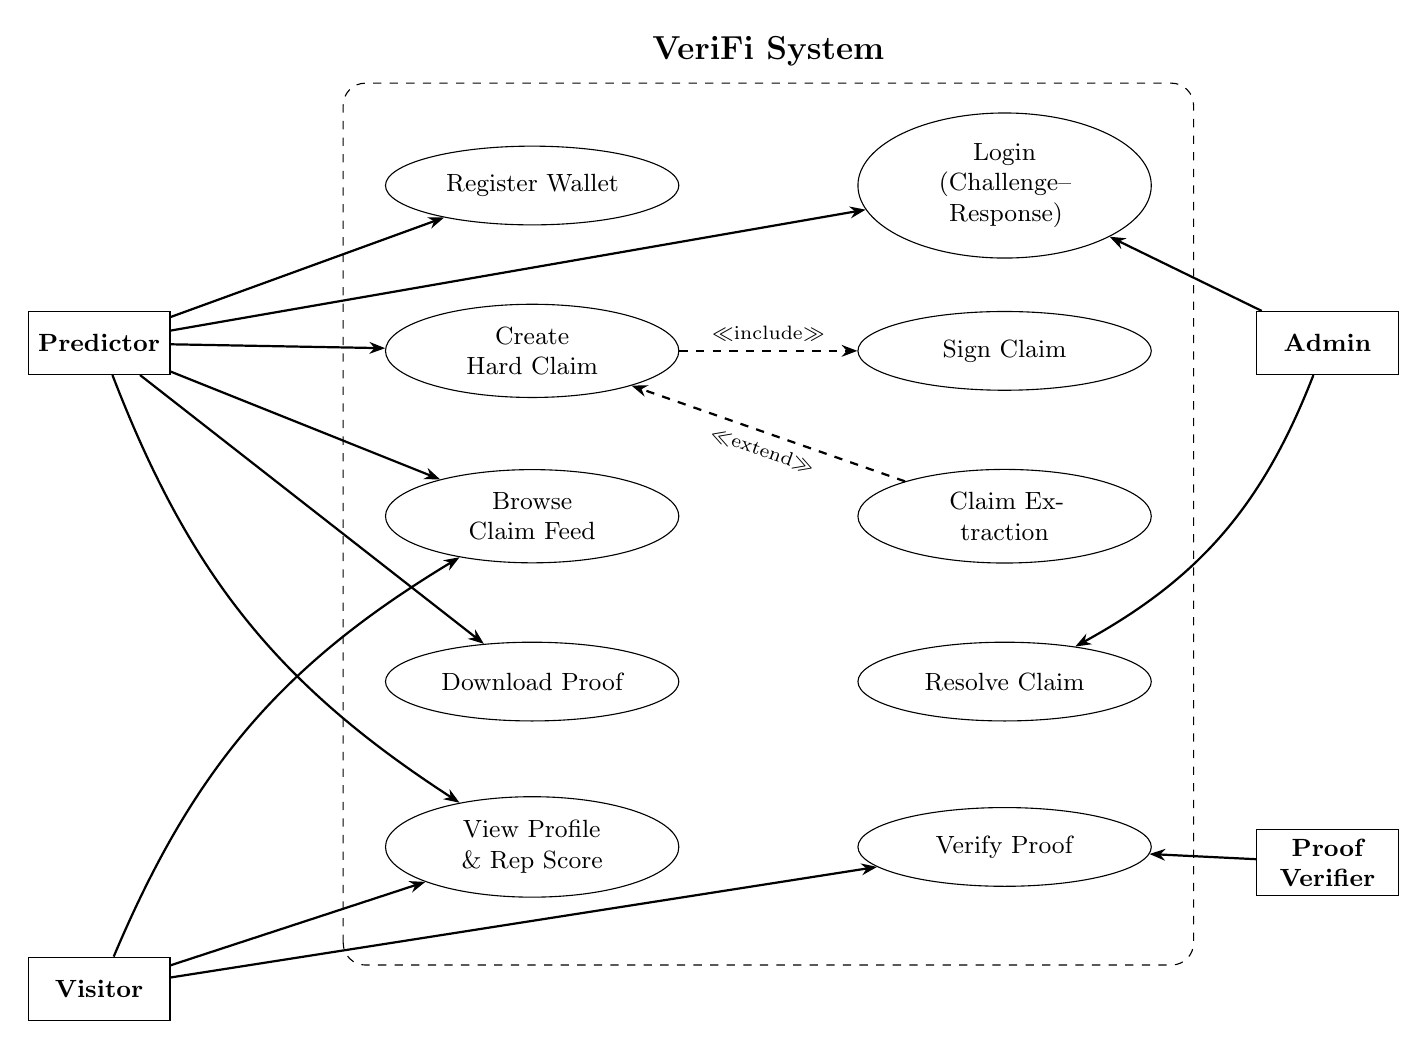
\begin{tikzpicture}[
    actor/.style={
        rectangle, minimum width=1.8cm, minimum height=0.8cm,
        draw, font=\small\bfseries, align=center
    },
    usecase/.style={
        ellipse, draw, minimum width=2.8cm, minimum height=1cm,
        font=\small, align=center, text width=2.4cm
    },
    arr/.style={-{Stealth[length=2mm]}, thick},
    dasharr/.style={-{Stealth[length=2mm]}, dashed, thick},
]

% System boundary (drawn explicitly so all use cases fit inside)
\draw[dashed, rounded corners=8pt] (0.9,-4.9) rectangle (11.7,6.3);
\node[font=\large\bfseries] at (6.3,6.7) {VeriFi System};

% Actors (left side)
\node[actor] (predictor) at (-2.2, 3.0)  {Predictor};
\node[actor] (visitor)   at (-2.2, -5.2) {Visitor};

% Actors (right side)
\node[actor] (admin)    at (13.4, 3.0)  {Admin};
\node[actor] (verifier) at (13.4, -3.6) {Proof\\Verifier};

% Use cases — left column
\node[usecase] (register) at (3.3, 5.0)  {Register Wallet};
\node[usecase] (create)   at (3.3, 2.9)  {Create Hard Claim};
\node[usecase] (feed)     at (3.3, 0.8)  {Browse Claim Feed};
\node[usecase] (download) at (3.3, -1.3) {Download Proof};
\node[usecase] (profile)  at (3.3, -3.4) {View Profile \& Rep Score};

% Use cases — right column
\node[usecase] (login)    at (9.3, 5.0)  {Login (Challenge--Response)};
\node[usecase] (sign)     at (9.3, 2.9)  {Sign Claim};
\node[usecase] (extract)  at (9.3, 0.8)  {Claim Extraction};
\node[usecase] (resolve)  at (9.3, -1.3) {Resolve Claim};
\node[usecase] (verify)   at (9.3, -3.4) {Verify Proof};

% Predictor associations
\draw[arr] (predictor) -- (register);
\draw[arr] (predictor) -- (login);
\draw[arr] (predictor) -- (create);
\draw[arr] (predictor) -- (feed);
\draw[arr] (predictor) -- (download);
\draw[arr] (predictor) to[bend right=18] (profile);

% Visitor associations
\draw[arr] (visitor) to[bend left=18] (feed);
\draw[arr] (visitor) -- (profile);
\draw[arr] (visitor) -- (verify);

% Admin associations
\draw[arr] (admin) -- (login);
\draw[arr] (admin) to[bend left=20] (resolve);

% Verifier associations
\draw[arr] (verifier) -- (verify);

% <<include>> / <<extend>> relationships
\draw[dasharr] (create) -- node[above, font=\scriptsize] {$\ll$include$\gg$} (sign);
\draw[dasharr] (extract) -- node[below, font=\scriptsize, sloped] {$\ll$extend$\gg$} (create);

\end{tikzpicture}%
}
\caption[Use Case Diagram]{UML use case diagram showing actor--system interactions.}
\label{fig:use_case}
\end{figure}

% ─────────────────────────────────────────────────────────────────────────────
\chapter{DESIGN}

\section{Information Structure}

The core data models and their relationships are described below.

\begin{table}[thbp]
\vskip\baselineskip
\caption[WalletUser Model]{\texttt{WalletUser} --- registered user identity.}
\begin{center}
\begin{tabular}{|l|l|p{7cm}|}
\hline
\textbf{Field} & \textbf{Type} & \textbf{Constraints} \\\hline
\texttt{id} & Auto PK & --- \\\hline
\texttt{address} & \texttt{CharField(42)} & Unique, lowercase Ethereum address (\texttt{0x} + 40 hex chars) \\\hline
\texttt{username} & \texttt{CharField(30)} & Unique; auto-derived from address if absent \\\hline
\texttt{avatar} & \texttt{CloudinaryField} & Optional profile image \\\hline
\texttt{rep} & \texttt{FloatField} & Reputation Score; default 200 \\\hline
\texttt{energy} & \texttt{FloatField} & Daily staking allowance; default 4, +3/day \\\hline
\texttt{created\_at} & \texttt{DateTimeField} & Auto-set on creation \\\hline
\end{tabular}
\label{table:walletuser_model}
\end{center}
\end{table}

\begin{table}[thbp]
\vskip\baselineskip
\caption[Asset Model]{\texttt{Asset} --- tradable financial asset with per-provider oracle symbol mapping.}
\begin{center}
\begin{tabular}{|l|l|p{6.2cm}|}
\hline
\textbf{Field} & \textbf{Type} & \textbf{Constraints} \\\hline
\texttt{id} & Auto PK & --- \\\hline
\texttt{name} & \texttt{CharField(100)} & e.g.\ ``Bitcoin'' \\\hline
\texttt{symbol} & \texttt{CharField(10)} & e.g.\ ``BTC'' \\\hline
\texttt{market\_type} & \texttt{CharField(20)} & \texttt{crypto} $\cdot$ \texttt{equity} $\cdot$ \texttt{forex} $\cdot$ \texttt{commodity} $\cdot$ \texttt{index} \\\hline
\texttt{provider\ symbols} & \texttt{CharField} $\times 5$ & Per-provider identifiers (Binance, KuCoin, Kraken, Twelve Data, CoinGecko/Yahoo) used by the oracle fallback chain \\\hline
\texttt{quote\_currency} & \texttt{CharField(10)} & e.g.\ USD, TRY \\\hline
\texttt{usage\_count} & \texttt{PositiveInteger} & Claim/position reference count; drives search ordering \\\hline
\end{tabular}
\label{table:asset_model}
\end{center}
\end{table}

\begin{table}[thbp]
\vskip\baselineskip
\caption[HardClaim Model]{\texttt{HardClaim} --- the canonical verifiable financial prediction entity.}
\begin{center}
\begin{tabular}{|l|l|p{6cm}|}
\hline
\textbf{Field} & \textbf{Type} & \textbf{Constraints} \\\hline
\texttt{id} & Auto PK & --- \\\hline
\texttt{author} & FK $\rightarrow$ \texttt{WalletUser} & Nullable (system claims) \\\hline
\texttt{post} & FK $\rightarrow$ \texttt{Post} & Optional originating post \\\hline
\texttt{channel} & FK $\rightarrow$ \texttt{Channel} & Optional channel scope \\\hline
\texttt{asset} & FK $\rightarrow$ \texttt{Asset} & Required \\\hline
\texttt{direction} & \texttt{CharField(20)} & \texttt{"Bullish"} or \texttt{"Bearish"} \\\hline
\texttt{value\_type} & \texttt{CharField(20)} & Percentage move vs.\ absolute price target \\\hline
\texttt{percentage} & \texttt{FloatField} & Move magnitude (or target price when \texttt{value\_type} is \texttt{PRICE}) \\\hline
\texttt{until} & \texttt{DateField} & Must be $>$ \texttt{created\_at} (DB constraint) \\\hline
\texttt{reference\_price} & \texttt{FloatField} & Entry price captured at creation \\\hline
\texttt{signature} & \texttt{TextField} & EIP-191 signature over the canonical payload \\\hline
\texttt{claim\_payload} & \texttt{JSONField} & Canonical signed JSON \\\hline
\texttt{status} & \texttt{CharField(12)} & \texttt{undetermined} (default) $\cdot$ \texttt{confirmed} $\cdot$ \texttt{rejected} \\\hline
\end{tabular}
\label{table:hardclaim_model}
\end{center}
\end{table}

\begin{table}[thbp]
\vskip\baselineskip
\caption[Position Model]{\texttt{Position} --- suggested trade tracked against market data.}
\begin{center}
\begin{tabular}{|p{4.4cm}|l|p{5.2cm}|}
\hline
\textbf{Field} & \textbf{Type} & \textbf{Constraints} \\\hline
\texttt{id} & Auto PK & --- \\\hline
\texttt{author} & FK $\rightarrow$ \texttt{WalletUser} & CASCADE delete \\\hline
\texttt{asset} & FK $\rightarrow$ \texttt{Asset} & Required \\\hline
\texttt{direction} & \texttt{CharField(10)} & \texttt{long} or \texttt{short} \\\hline
\texttt{entry\_price} & \texttt{FloatField} & Price at which the position activates \\\hline
\texttt{stop\_loss}, \texttt{take\_profit} & \texttt{FloatField} & Exit thresholds \\\hline
\texttt{lifetime} & \texttt{DateTimeField} & Expiry of the position \\\hline
\texttt{exit\_price}, \texttt{pnl\_percentage} & \texttt{FloatField} & Set at resolution \\\hline
\texttt{signature}, \texttt{position\_payload} & \texttt{Text}/\texttt{JSON} & EIP-191 signed canonical payload \\\hline
\texttt{status} & \texttt{CharField(20)} & \texttt{pending} $\cdot$ \texttt{active} $\cdot$ \texttt{missed} $\cdot$ \texttt{confirmed} $\cdot$ \texttt{rejected} $\cdot$ \texttt{expired} $\cdot$ \texttt{closed\_early} \\\hline
\end{tabular}
\label{table:position_model}
\end{center}
\end{table}

\begin{table}[thbp]
\vskip\baselineskip
\caption[ClaimMarket and ClaimStake Models]{\texttt{ClaimMarket} and \texttt{ClaimStake} --- the CPMM reputation market ledger.}
\begin{center}
\begin{tabular}{|p{4.6cm}|l|p{5cm}|}
\hline
\textbf{Field} & \textbf{Type} & \textbf{Constraints} \\\hline
\texttt{hard\_claim} & 1:1 $\rightarrow$ \texttt{HardClaim} & PK; one market per claim \\\hline
\texttt{y\_reserve}, \texttt{n\_reserve} & \texttt{FloatField} & CPMM reserves \\\hline
\texttt{escrow}, \texttt{total\_burned} & \texttt{FloatField} & Rep held / burned in fees \\\hline
\texttt{creator\_side}, \texttt{creator\_stake\_rep} & --- & Creator's own position (10--100 rep) \\\hline
\texttt{resolved}, \texttt{refunded\_trivial} & \texttt{Boolean} & Lifecycle flags \\\hline
\hline
\texttt{market}, \texttt{user} & FKs & Unique together; one stake per user per claim \\\hline
\texttt{side} & \texttt{CharField(3)} & \texttt{YES} or \texttt{NO} \\\hline
\texttt{rep\_paid\_gross/net} & \texttt{FloatField} & 10 rep gross; net after 5\% burn \\\hline
\texttt{shares}, \texttt{entry\_price} & \texttt{FloatField} & Locked payout receipt \\\hline
\end{tabular}
\label{table:market_model}
\end{center}
\end{table}

\begin{sloppypar}
In addition to the entities above, the final schema includes: \texttt{Post} (free-form social post with image attachment), \texttt{PostLike}, \texttt{PostComment} (nested, with likes), \texttt{Channel} and \texttt{ChannelMembership} (sub-communities with \texttt{owner}/\texttt{moderator}/\texttt{member} roles and posting permissions), \texttt{Follow} (asymmetric user follows), \texttt{Notification}, \texttt{SavedProof}, \texttt{HardClaimEvent} and \texttt{PositionEvent} (append-only audit logs of every creation, price check, and resolution), \texttt{OHLCData} (cached oracle candles), and \texttt{AssetSubscription} (observer-pattern registrations linking expiring claims to the resolution engine).
\end{sloppypar}

\begin{figure}[H]
\centering
\resizebox{0.95\textwidth}{!}{%
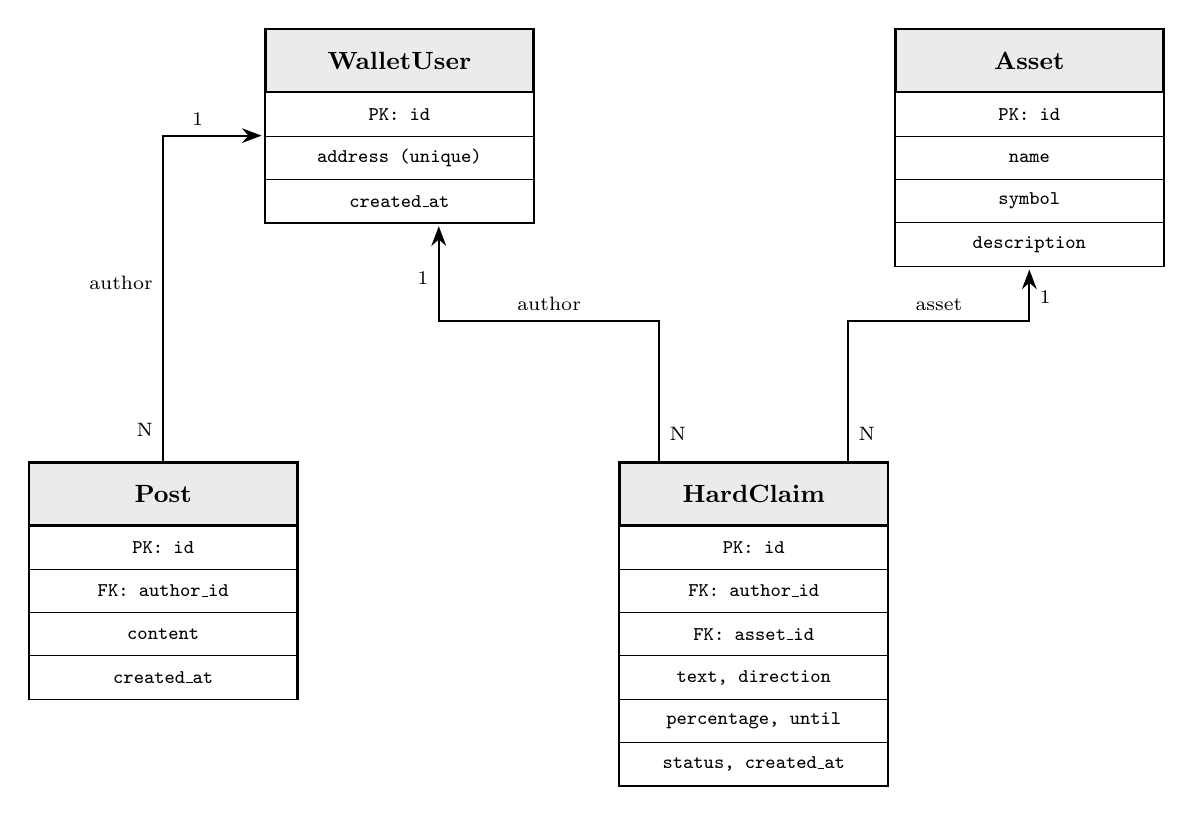
\begin{tikzpicture}[
    entity/.style={
        rectangle, draw, thick, minimum width=3.4cm, minimum height=0.8cm,
        font=\small\bfseries, fill=black!8
    },
    attr/.style={
        rectangle, draw, thin, minimum width=3.4cm, minimum height=0.55cm,
        font=\scriptsize\ttfamily, anchor=north
    },
]

% WalletUser entity (top-left)
\node[entity] (wu) at (0, 0) {WalletUser};
\node[attr] (wu1) at (0, -0.4) {PK: id};
\node[attr] (wu2) at (0, -0.95) {address (unique)};
\node[attr] (wu3) at (0, -1.5) {created\_at};
\node[draw, thin, fit=(wu)(wu1)(wu2)(wu3), inner sep=0pt] {};

% Asset entity (top-right)
\node[entity] (asset) at (8, 0) {Asset};
\node[attr] (a1) at (8, -0.4)  {PK: id};
\node[attr] (a2) at (8, -0.95) {name};
\node[attr] (a3) at (8, -1.5)  {symbol};
\node[attr] (a4) at (8, -2.05) {description};
\node[draw, thin, fit=(asset)(a1)(a2)(a3)(a4), inner sep=0pt] {};

% Post (Legacy) entity (bottom-left)
\node[entity] (post) at (-3, -5.5) {Post};
\node[attr] (p1) at (-3, -5.9)  {PK: id};
\node[attr] (p2) at (-3, -6.45) {FK: author\_id};
\node[attr] (p3) at (-3, -7.0)  {content};
\node[attr] (p4) at (-3, -7.55) {created\_at};
\node[draw, thin, fit=(post)(p1)(p2)(p3)(p4), inner sep=0pt] {};

% HardClaim entity (bottom-right)
\node[entity] (hc) at (4.5, -5.5) {HardClaim};
\node[attr] (hc1) at (4.5, -5.9) {PK: id};
\node[attr] (hc2) at (4.5, -6.45) {FK: author\_id};
\node[attr] (hc3) at (4.5, -7.0) {FK: asset\_id};
\node[attr] (hc4) at (4.5, -7.55) {text, direction};
\node[attr] (hc5) at (4.5, -8.1) {percentage, until};
\node[attr] (hc6) at (4.5, -8.65) {status, created\_at};
\node[draw, thin, fit=(hc)(hc1)(hc2)(hc3)(hc4)(hc5)(hc6), inner sep=0pt] {};

% Post.author -> WalletUser (up, then into the left edge of the box)
\draw[thick, -{Stealth[length=2.5mm]}]
    (-3, -5.1) -- node[left, font=\scriptsize, pos=0.1] {N}
                  node[left, font=\scriptsize, pos=0.55] {author}
    (-3, -0.95)
    -- node[above, font=\scriptsize, pos=0.35] {1} (-1.75, -0.95);

% HardClaim.author -> WalletUser (L-shaped, ends at box bottom edge)
\draw[thick, -{Stealth[length=2.5mm]}]
    (3.3, -5.1) -- node[right, font=\scriptsize, pos=0.2] {N}  (3.3, -3.3)
    -- node[above, font=\scriptsize] {author} (0.5, -3.3)
    -- node[left, font=\scriptsize, pos=0.45] {1} (0.5, -2.1);

% HardClaim.asset -> Asset (L-shaped, ends at box bottom edge)
\draw[thick, -{Stealth[length=2.5mm]}]
    (5.7, -5.1) -- node[right, font=\scriptsize, pos=0.2] {N} (5.7, -3.3)
    -- node[above, font=\scriptsize] {asset} (8, -3.3)
    -- node[right, font=\scriptsize, pos=0.45] {1} (8, -2.65);

\end{tikzpicture}%
}
\caption[Entity-Relationship Diagram]{Entity-Relationship diagram of the core data models. \texttt{HardClaim} references both \texttt{WalletUser} (author) and \texttt{Asset}. \texttt{Post} also references \texttt{WalletUser}. Only the core entities are shown; the full schema is listed in the text above.}
\label{fig:er_diagram}
\end{figure}

\section{Information Flow}

\textbf{Authentication flow (native wallet):} The browser generates a mnemonic and derives a secp256k1 key pair entirely client-side. The address is registered with the backend via \texttt{POST /api/auth/register/}. On login, the browser requests a nonce from \texttt{GET /api/auth/challenge/}, signs it with the private key (EIP-191), and sends the signature to \texttt{POST /api/auth/login/}. The backend uses \texttt{eth\_account.recover\_message()} to recover the signing address and issues a JWT on match.

\textbf{Claim creation flow:} An authenticated user composes a post; the rule-based extractor runs live while typing and proposes Claim Cards, or the user fills the structured claim form directly. The client signs the canonical claim payload with the wallet's private key (EIP-191) and sends \texttt{POST /api/posts/hard-claims/} with a Bearer JWT header. The backend validates the JWT, recovers the signer address from the signature and rejects mismatches, checks payload consistency and timestamp freshness ($\pm$5 minutes, anti-replay), validates all claim fields, captures the reference price from an intraday quote, opens the CPMM reputation market with the creator's stake, and stores the record with status \texttt{undetermined}.

\textbf{Claim resolution flow:} When a claim's \texttt{until} date passes (or an early target hit is detected during a price check), the resolution engine fetches OHLC candles for the claim window through the provider fallback chain, determines whether the target was reached at any point after creation, sets the status to \texttt{confirmed} or \texttt{rejected}, writes a \texttt{HardClaimEvent} audit record with the price evidence, and settles the reputation market: winning stakes receive their locked payout, the creator cut is applied, and trivial markets are refunded. Manual admin resolution via \texttt{PATCH /api/}\allowbreak\texttt{posts/hard-claims/}\allowbreak\texttt{\{id\}/update-status/} remains as a fallback. Expiring claims are connected to the engine through an observer pattern (\texttt{AssetSubscription}), so price data fetched once per asset resolves all subscribed claims.

% --- Sequence Diagram 1: Native Wallet Registration & Login ---
\begin{figure}[H]
\centering
\resizebox{\textwidth}{!}{%
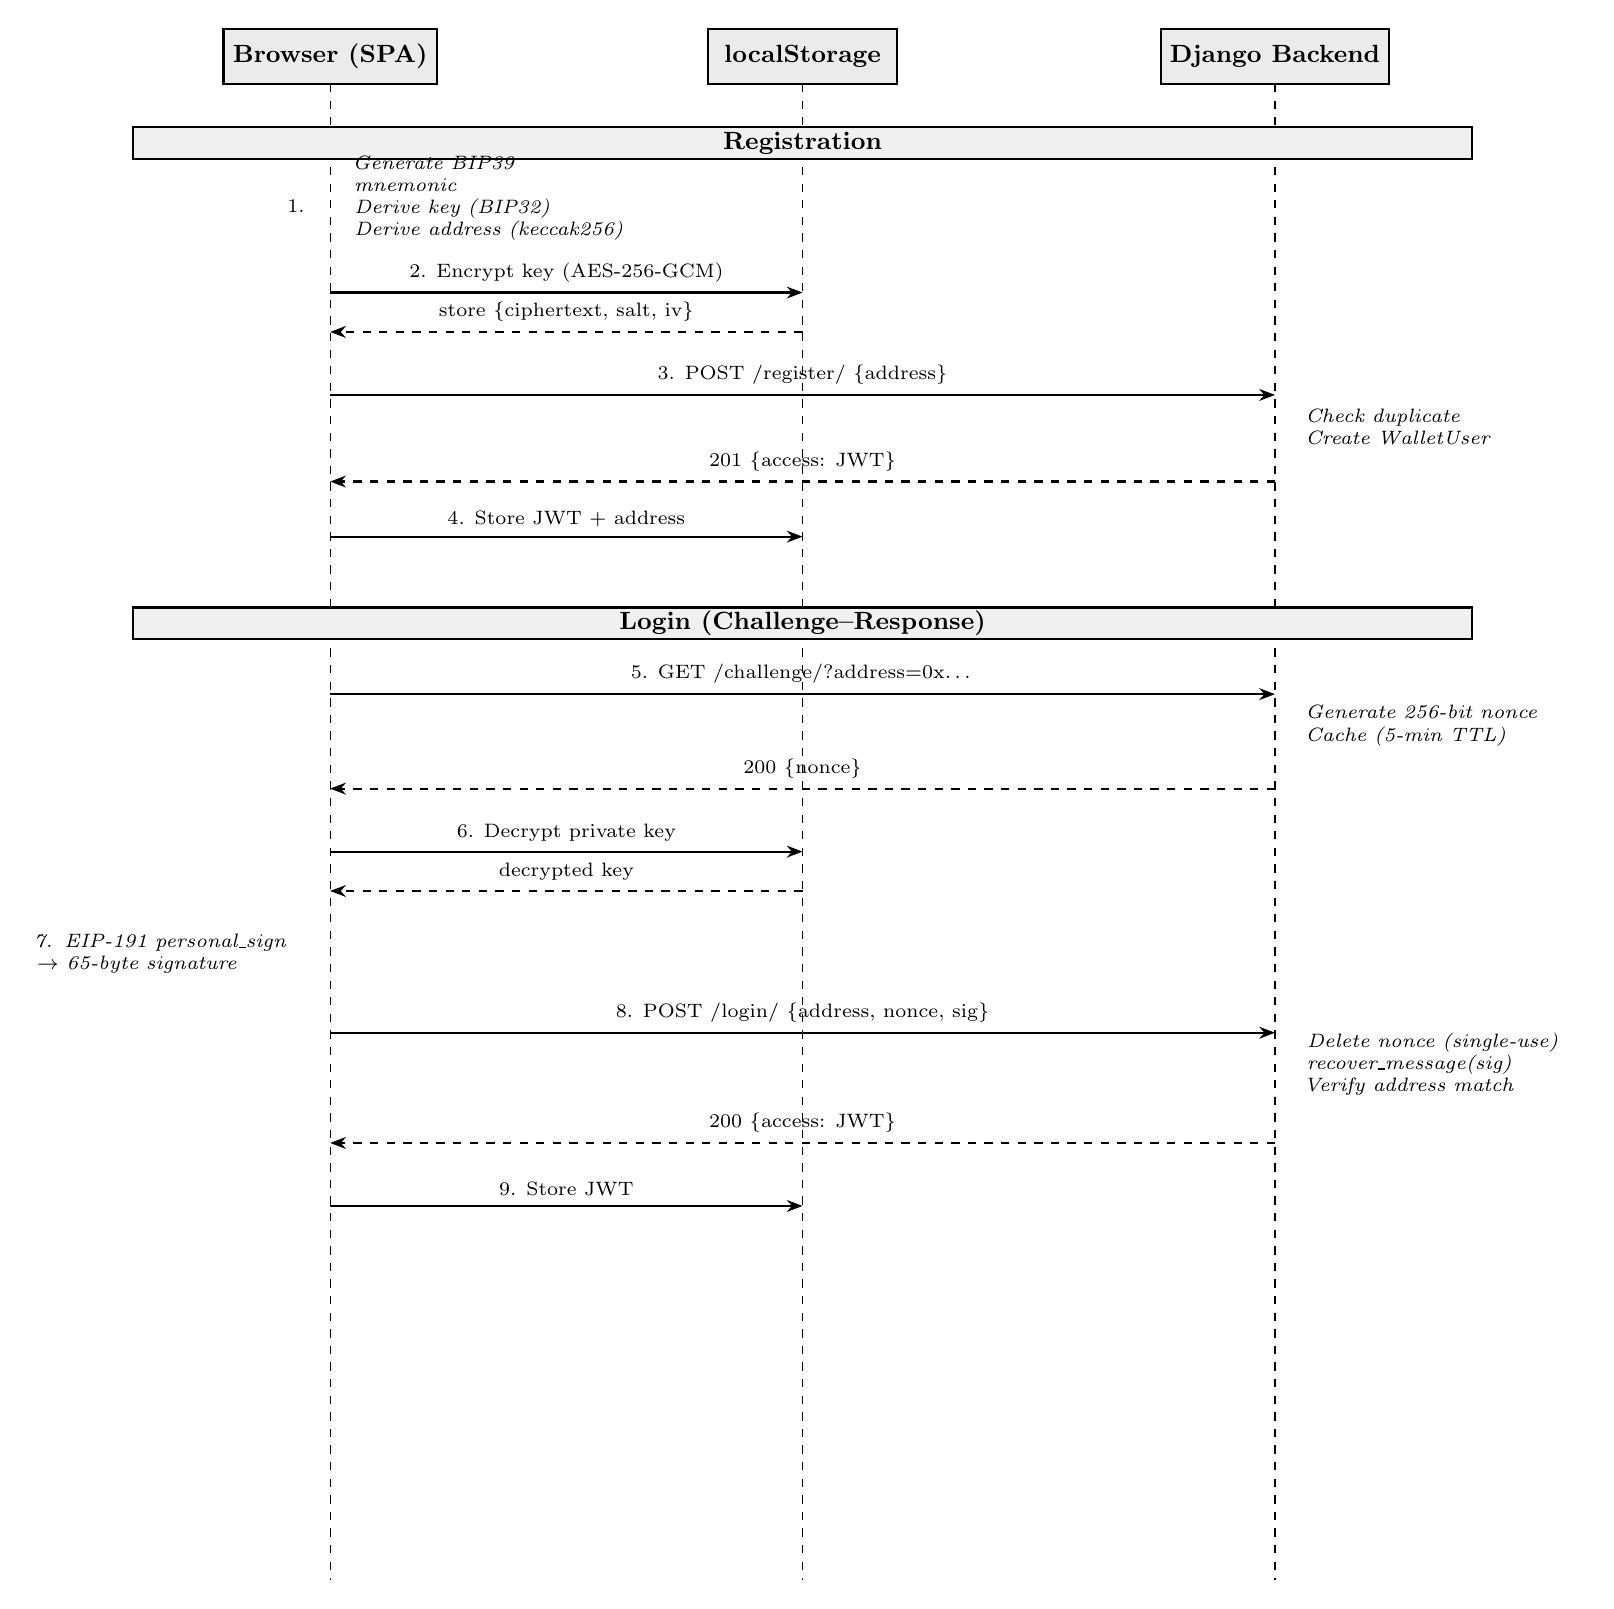
\begin{tikzpicture}[
    arr/.style={-{Stealth[length=2mm]}, thick},
    msg/.style={font=\scriptsize},
    note/.style={font=\scriptsize\itshape, text width=3.4cm, align=left},
    header/.style={rectangle, draw, thick, fill=black!8, minimum width=2.4cm, minimum height=0.7cm, font=\small\bfseries},
]
% Lifelines
\node[header] (bh) at (0,0) {Browser (SPA)};
\node[header] (lh) at (6,0) {localStorage};
\node[header] (sh) at (12,0) {Django Backend};

\draw[dashed] (0,-0.35) -- ++(0,-19);
\draw[dashed] (6,-0.35) -- ++(0,-19);
\draw[dashed] (12,-0.35) -- ++(0,-19);

% --- Registration ---
\draw[thick, fill=black!6] (-2.5,-0.9) rectangle (14.5,-1.3);
\node[font=\small\bfseries] at (6,-1.1) {Registration};

% 1
\node[msg, anchor=east] at (-0.2,-1.9) {1.};
\node[note, anchor=west] at (0.2,-1.8) {Generate BIP39 mnemonic\\Derive key (BIP32)\\Derive address (keccak256)};

% 2
\draw[arr] (0,-3.0) -- node[msg, above] {2. Encrypt key (AES-256-GCM)} (6,-3.0);
\draw[arr, dashed] (6,-3.5) -- node[msg, above] {store \{ciphertext, salt, iv\}} (0,-3.5);

% 3
\draw[arr] (0,-4.3) -- node[msg, above] {3. POST /register/ \{address\}} (12,-4.3);
\node[note, anchor=west] at (12.3,-4.7) {Check duplicate\\Create WalletUser};
\draw[arr, dashed] (12,-5.4) -- node[msg, above] {201 \{access: JWT\}} (0,-5.4);

% 4
\draw[arr] (0,-6.1) -- node[msg, above] {4. Store JWT + address} (6,-6.1);

% --- Login ---
\draw[thick, fill=black!6] (-2.5,-7.0) rectangle (14.5,-7.4);
\node[font=\small\bfseries] at (6,-7.2) {Login (Challenge--Response)};

% 5
\draw[arr] (0,-8.1) -- node[msg, above] {5. GET /challenge/?address=0x\ldots} (12,-8.1);
\node[note, anchor=west] at (12.3,-8.5) {Generate 256-bit nonce\\Cache (5-min TTL)};
\draw[arr, dashed] (12,-9.3) -- node[msg, above] {200 \{nonce\}} (0,-9.3);

% 6
\draw[arr] (0,-10.1) -- node[msg, above] {6. Decrypt private key} (6,-10.1);
\draw[arr, dashed] (6,-10.6) -- node[msg, above] {decrypted key} (0,-10.6);

% 7
\node[note, anchor=east] at (-0.2,-11.4) {7. EIP-191 personal\_sign\\$\rightarrow$ 65-byte signature};

% 8
\draw[arr] (0,-12.4) -- node[msg, above] {8. POST /login/ \{address, nonce, sig\}} (12,-12.4);
\node[note, anchor=west] at (12.3,-12.8) {Delete nonce (single-use)\\recover\_message(sig)\\Verify address match};
\draw[arr, dashed] (12,-13.8) -- node[msg, above] {200 \{access: JWT\}} (0,-13.8);

% 9
\draw[arr] (0,-14.6) -- node[msg, above] {9. Store JWT} (6,-14.6);

\end{tikzpicture}%
}
\caption[Native Wallet Sequence Diagram]{Sequence diagram for native wallet registration and challenge--response login.}
\label{fig:seq_native}
\end{figure}

% --- Sequence Diagram 2: MetaMask Registration & Login ---
\begin{figure}[H]
\centering
\resizebox{\textwidth}{!}{%
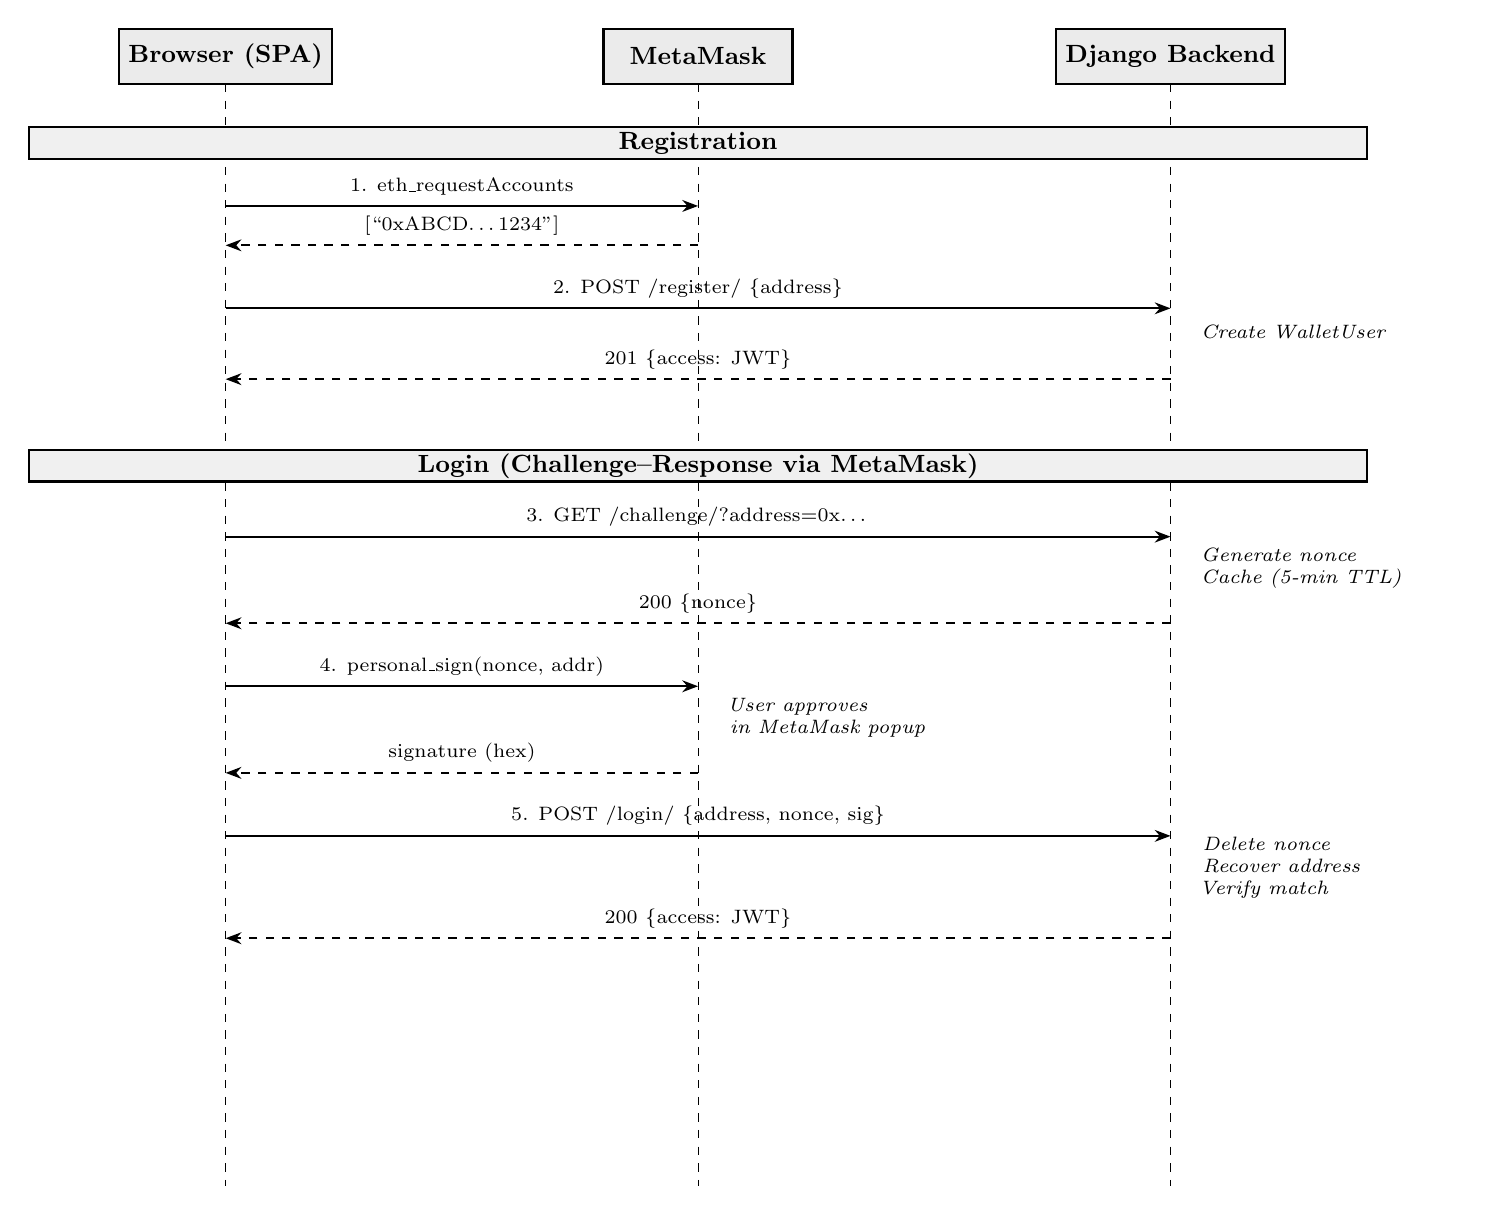
\begin{tikzpicture}[
    arr/.style={-{Stealth[length=2mm]}, thick},
    msg/.style={font=\scriptsize},
    note/.style={font=\scriptsize\itshape, text width=3.4cm, align=left},
    header/.style={rectangle, draw, thick, fill=black!8, minimum width=2.4cm, minimum height=0.7cm, font=\small\bfseries},
]
% Lifelines
\node[header] (bh) at (0,0) {Browser (SPA)};
\node[header] (mh) at (6,0) {MetaMask};
\node[header] (sh) at (12,0) {Django Backend};

\draw[dashed] (0,-0.35) -- ++(0,-14);
\draw[dashed] (6,-0.35) -- ++(0,-14);
\draw[dashed] (12,-0.35) -- ++(0,-14);

% --- Registration ---
\draw[thick, fill=black!6] (-2.5,-0.9) rectangle (14.5,-1.3);
\node[font=\small\bfseries] at (6,-1.1) {Registration};

\draw[arr] (0,-1.9) -- node[msg, above] {1. eth\_requestAccounts} (6,-1.9);
\draw[arr, dashed] (6,-2.4) -- node[msg, above] {[``0xABCD\ldots1234'']} (0,-2.4);

\draw[arr] (0,-3.2) -- node[msg, above] {2. POST /register/ \{address\}} (12,-3.2);
\node[note, anchor=west] at (12.3,-3.5) {Create WalletUser};
\draw[arr, dashed] (12,-4.1) -- node[msg, above] {201 \{access: JWT\}} (0,-4.1);

% --- Login ---
\draw[thick, fill=black!6] (-2.5,-5.0) rectangle (14.5,-5.4);
\node[font=\small\bfseries] at (6,-5.2) {Login (Challenge--Response via MetaMask)};

\draw[arr] (0,-6.1) -- node[msg, above] {3. GET /challenge/?address=0x\ldots} (12,-6.1);
\node[note, anchor=west] at (12.3,-6.5) {Generate nonce\\Cache (5-min TTL)};
\draw[arr, dashed] (12,-7.2) -- node[msg, above] {200 \{nonce\}} (0,-7.2);

\draw[arr] (0,-8.0) -- node[msg, above] {4. personal\_sign(nonce, addr)} (6,-8.0);
\node[note, anchor=west] at (6.3,-8.4) {User approves\\in MetaMask popup};
\draw[arr, dashed] (6,-9.1) -- node[msg, above] {signature (hex)} (0,-9.1);

\draw[arr] (0,-9.9) -- node[msg, above] {5. POST /login/ \{address, nonce, sig\}} (12,-9.9);
\node[note, anchor=west] at (12.3,-10.3) {Delete nonce\\Recover address\\Verify match};
\draw[arr, dashed] (12,-11.2) -- node[msg, above] {200 \{access: JWT\}} (0,-11.2);

\end{tikzpicture}%
}
\caption[MetaMask Sequence Diagram]{Sequence diagram for MetaMask registration and login. The private key never leaves the MetaMask vault.}
\label{fig:seq_metamask}
\end{figure}

% --- Sequence Diagram 3: Hard Claim Creation ---
\begin{figure}[H]
\centering
\resizebox{\textwidth}{!}{%
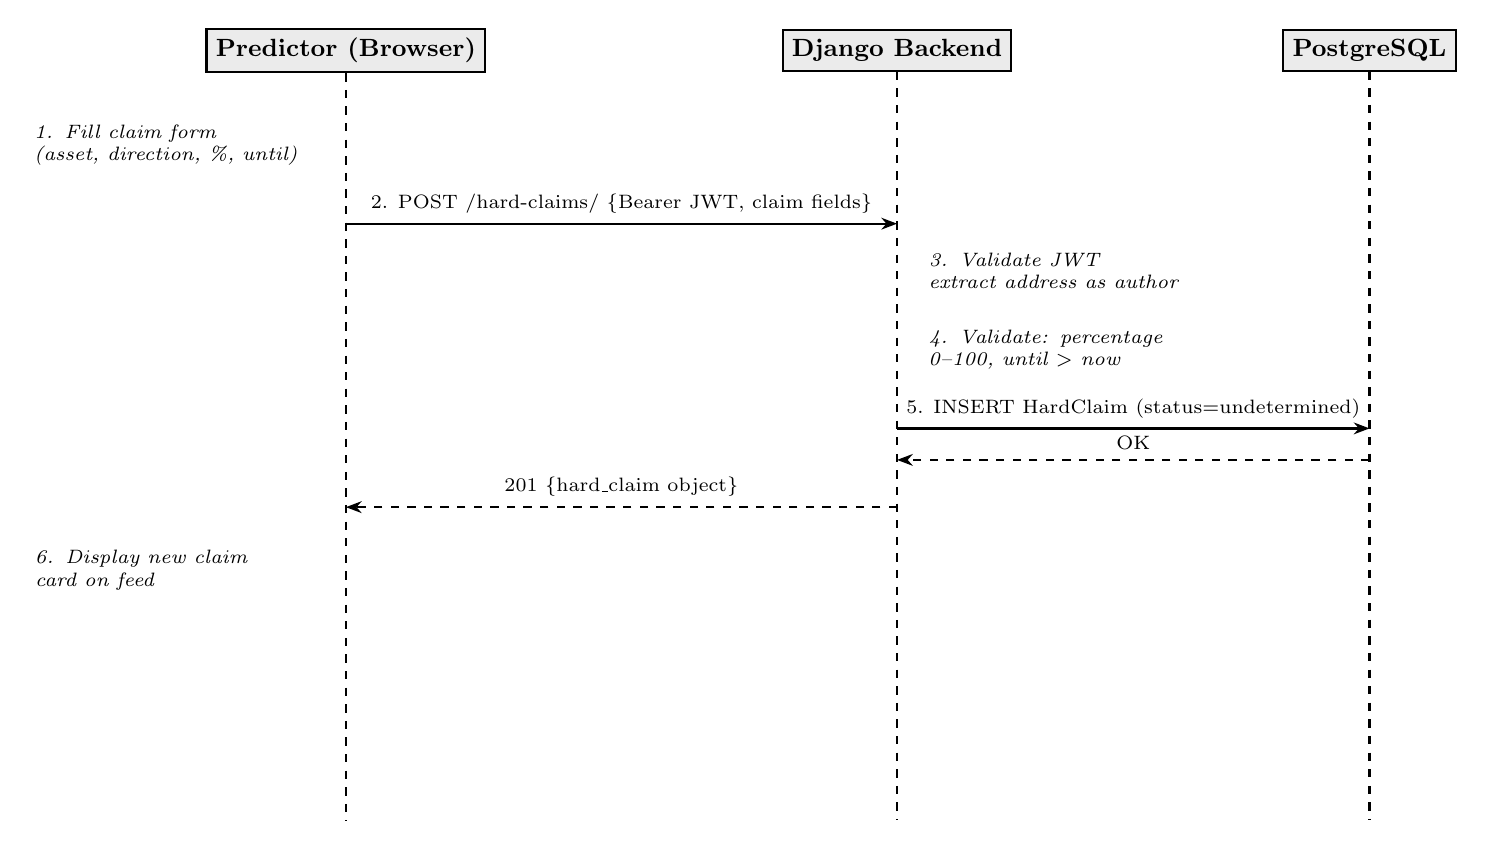
\begin{tikzpicture}[
    arr/.style={-{Stealth[length=2mm]}, thick},
    msg/.style={font=\scriptsize},
    note/.style={font=\scriptsize\itshape, text width=3.5cm, align=left},
]
% Lifelines
\node[rectangle, draw, thick, fill=black!8, minimum width=2.6cm, font=\small\bfseries] (uh) at (0,0) {Predictor (Browser)};
\node[rectangle, draw, thick, fill=black!8, minimum width=2.2cm, font=\small\bfseries] (sh) at (7,0) {Django Backend};
\node[rectangle, draw, thick, fill=black!8, minimum width=2.2cm, font=\small\bfseries] (dh) at (13,0) {PostgreSQL};

\draw[dashed, thick] (uh.south) -- ++(0,-9.5);
\draw[dashed, thick] (sh.south) -- ++(0,-9.5);
\draw[dashed, thick] (dh.south) -- ++(0,-9.5);

% 1. Fill form
\node[note, anchor=east] at (-0.3,-1.2) {1. Fill claim form\\(asset, direction, \%, until)};

% 2. POST
\draw[arr] (0,-2.2) -- node[msg, above] {2. POST /hard-claims/ \{Bearer JWT, claim fields\}} (7,-2.2);

% 3-4. Validate
\node[note, anchor=west] at (7.3,-2.8) {3. Validate JWT\\extract address as author};
\node[note, anchor=west] at (7.3,-3.8) {4. Validate: percentage\\0--100, until $>$ now};

% 5. Insert
\draw[arr] (7,-4.8) -- node[msg, above] {5. INSERT HardClaim (status=undetermined)} (13,-4.8);
\draw[arr, dashed] (13,-5.2) -- node[msg, above] {OK} (7,-5.2);

% Response
\draw[arr, dashed] (7,-5.8) -- node[msg, above] {201 \{hard\_claim object\}} (0,-5.8);

% 6. Display
\node[note, anchor=east] at (-0.3,-6.6) {6. Display new claim\\card on feed};

\end{tikzpicture}%
}
\caption[Hard Claim Creation Sequence]{Sequence diagram for hard claim creation. The backend validates all fields and stores the claim with initial status \texttt{undetermined}.}
\label{fig:seq_claim}
\end{figure}

\section{System Design}

The system follows a strict client-server separation. The frontend is a static SPA deployed on Vercel that communicates with the backend exclusively through the REST API over HTTPS. The backend is stateless: all authenticated state is in the JWT token carried by the client. The private key never leaves the browser.

The REST API is organized into three Django apps:
\begin{sloppypar}
\begin{itemize}
    \item \texttt{accounts} --- authentication, profiles, follows, and energy: \texttt{/api/auth/register/}, \texttt{/api/auth/challenge/}, \texttt{/api/auth/login/}, profile and follow endpoints
    \item \texttt{posts} --- content and markets: posts, comments, likes, hard claims, positions, channels, assets and asset search, claim extraction, reputation market stakes, proofs, charts, and search
    \item \texttt{notifications} --- per-user notification feed with mark-as-read and delete
\end{itemize}
\end{sloppypar}

API errors follow a uniform envelope \texttt{\{error: \{code, message, fields\}\}} so the frontend can pin validation messages to the offending form field.

\begin{sloppypar}
Cross-origin requests from the frontend origin (Vercel domain and \texttt{localhost:5173} in development) are handled by \texttt{django-cors-headers}.
\end{sloppypar}

\begin{figure}[H]
\centering
\resizebox{\textwidth}{!}{%
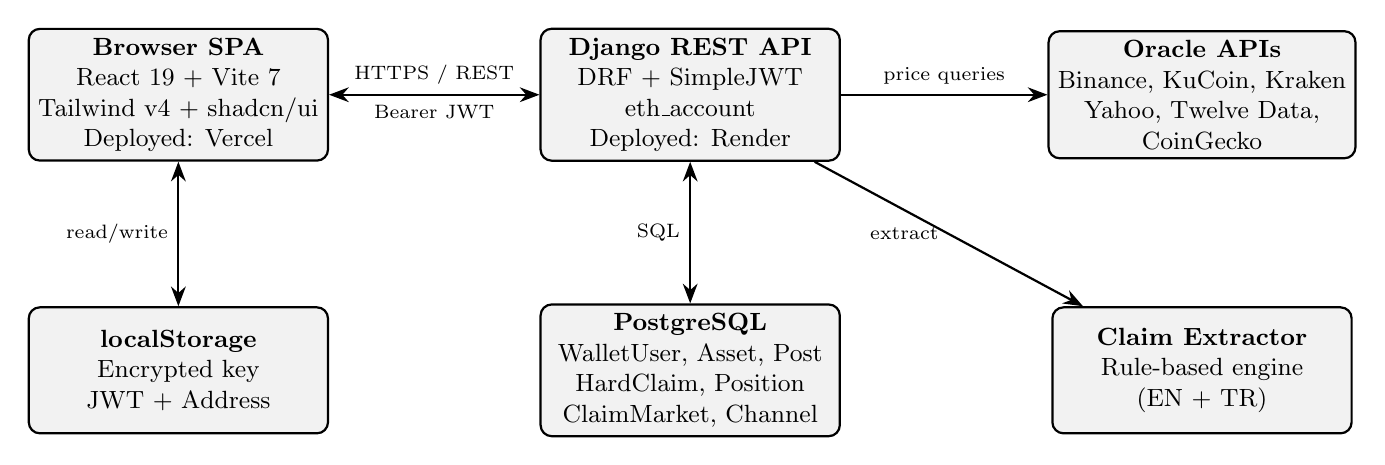
\begin{tikzpicture}[
    comp/.style={
        rectangle, draw, thick, rounded corners=4pt,
        minimum width=3.8cm, minimum height=1.6cm,
        font=\small, align=center, fill=black!5
    },
    arr/.style={-{Stealth[length=2.5mm]}, thick},
    darr/.style={{Stealth[length=2.5mm]}-{Stealth[length=2.5mm]}, thick},
]

% Row 1: main components
\node[comp] (frontend) at (0, 0)
    {\textbf{Browser SPA}\\React 19 + Vite 7\\Tailwind v4 + shadcn/ui\\Deployed: Vercel};

\node[comp] (backend) at (6.5, 0)
    {\textbf{Django REST API}\\DRF + SimpleJWT\\eth\_account\\Deployed: Render};

\node[comp] (oracle) at (13, 0)
    {\textbf{Oracle APIs}\\Binance, KuCoin, Kraken\\Yahoo, Twelve Data,\\CoinGecko};

% Row 2: storage and services
\node[comp] (local) at (0, -3.5)
    {\textbf{localStorage}\\Encrypted key\\JWT + Address};

\node[comp] (db) at (6.5, -3.5)
    {\textbf{PostgreSQL}\\WalletUser, Asset, Post\\HardClaim, Position\\ClaimMarket, Channel};

\node[comp] (llm) at (13, -3.5)
    {\textbf{Claim Extractor}\\Rule-based engine\\(EN + TR)};

% Arrows
\draw[darr] (frontend) -- node[above, font=\scriptsize] {HTTPS / REST} node[below, font=\scriptsize] {Bearer JWT} (backend);
\draw[darr] (frontend) -- node[left, font=\scriptsize] {read/write} (local);
\draw[darr] (backend) -- node[left, font=\scriptsize] {SQL} (db);
\draw[arr] (backend) -- node[above, font=\scriptsize] {price queries} (oracle);
\draw[arr] (backend) -- node[left, font=\scriptsize] {extract} (llm);

\end{tikzpicture}%
}
\caption[System Architecture]{High-level system architecture. The frontend communicates with the stateless backend over HTTPS; the private key never leaves the browser.}
\label{fig:architecture}
\end{figure}

\section{Authentication Design}
\label{sec:auth_design}

The authentication system is designed around the invariant that the private key is never transmitted to or stored by the server. The server only sees a wallet address (a 20-byte Keccak-256 hash of a public key) and a cryptographic signature over a server-issued nonce.

The native VeriFi wallet uses BIP39 (12-word mnemonic, 128 bits of entropy), BIP32/BIP44 key derivation (path \texttt{m/44'/60'/0'/0/0}), and standard Ethereum address derivation. The private key is encrypted with AES-256-GCM using a key derived from the user's passphrase via PBKDF2-SHA256 (100,000 iterations) and stored as a JSON ciphertext object in browser \texttt{localStorage}.

Login uses EIP-191 personal\_sign: the server generates a random hex nonce (32 bytes, 5-minute TTL, single-use), the client signs it, and the server uses \texttt{eth\_account.recover\_message()} to verify the signature. The following table summarises the security properties of both wallet modes.

\begin{table}[thbp]
\vskip\baselineskip
\caption[Authentication Security Properties]{Security properties of native wallet vs.\ MetaMask authentication.}
\begin{center}
\begin{tabular}{|p{3.5cm}|p{4.8cm}|p{3.8cm}|}
\hline
\textbf{Property} & \textbf{Native Wallet} & \textbf{MetaMask} \\\hline
Private key location & \texttt{localStorage} (AES-256-GCM encrypted) & MetaMask encrypted vault \\\hline
Private key transmitted? & Never & Never \\\hline
Replay attack protection & Single-use nonce (5-min TTL) & Single-use nonce (5-min TTL) \\\hline
Signature scheme & EIP-191 personal\_sign (secp256k1) & EIP-191 personal\_sign (secp256k1) \\\hline
Session mechanism & Stateless JWT (7-day expiry) & Stateless JWT (7-day expiry) \\\hline
\end{tabular}
\label{table:auth_security}
\end{center}
\end{table}

Figure~\ref{fig:login_flowchart} presents the combined authentication flowchart, showing how the system routes a user through either the native wallet or MetaMask path before converging on the shared challenge--response verification.

\begin{figure}[p]
\centering
\resizebox{0.85\textwidth}{!}{%
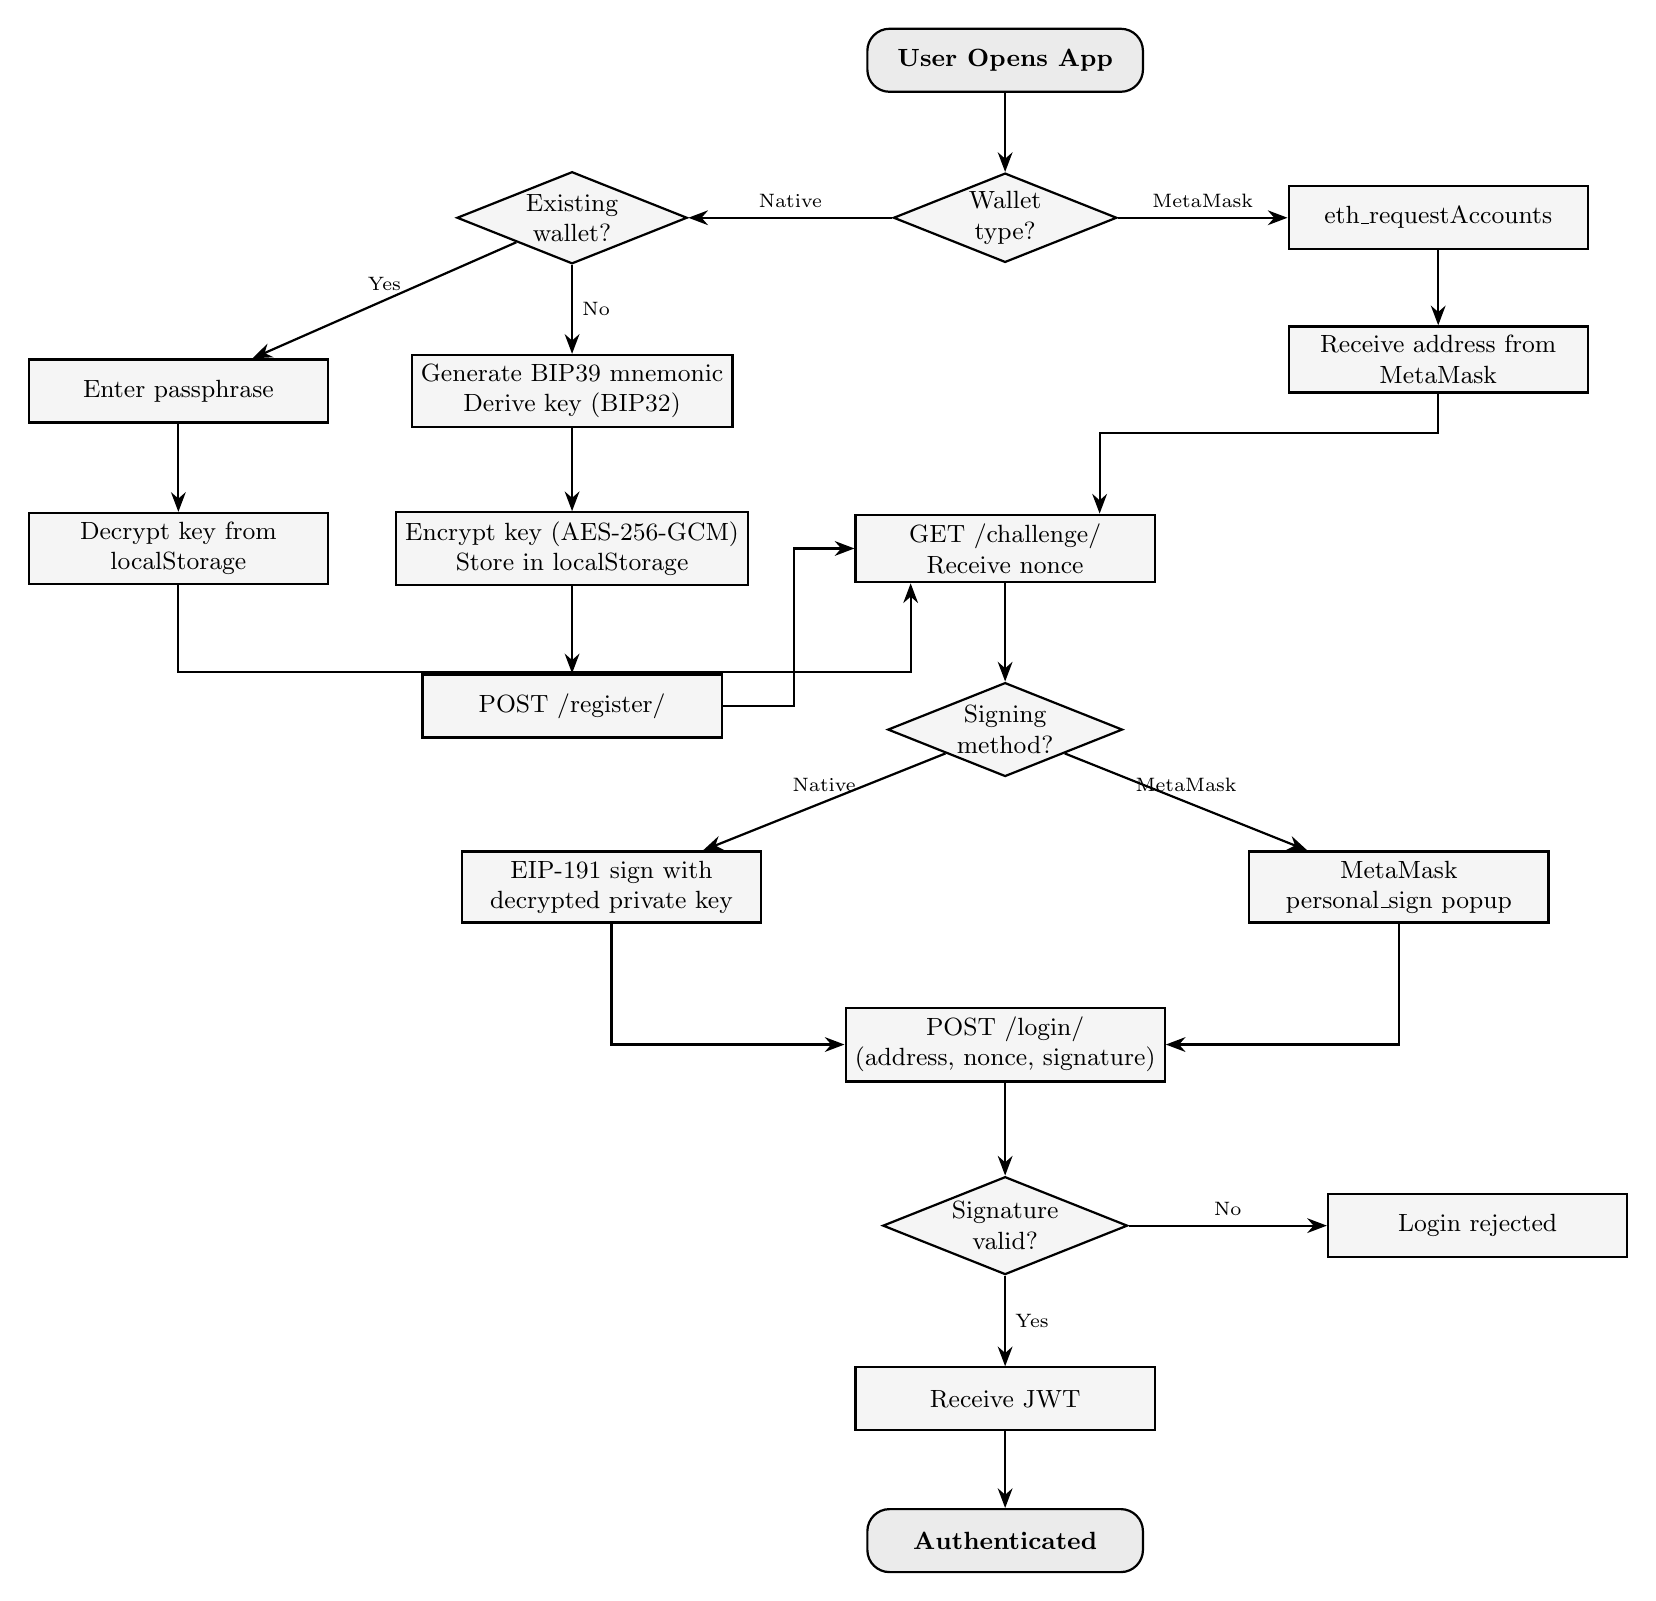
\begin{tikzpicture}[
    startstop/.style={
        rectangle, rounded corners=8pt, draw, thick,
        minimum width=3.5cm, minimum height=0.8cm,
        font=\small\bfseries, fill=black!8
    },
    process/.style={
        rectangle, draw, thick,
        minimum width=3.8cm, minimum height=0.8cm,
        font=\small, align=center, fill=black!4
    },
    decision/.style={
        diamond, draw, thick, aspect=2.5,
        font=\small, align=center, fill=black!4,
        inner sep=1pt
    },
    arr/.style={-{Stealth[length=2.5mm]}, thick},
]

% Start
\node[startstop] (start) at (0, 0) {User Opens App};

% Decision: wallet type
\node[decision] (wallettype) at (0, -2) {Wallet\\type?};

% ============ MetaMask branch (RIGHT) ============
\node[process] (mmreq) at (5.5, -2) {eth\_requestAccounts};
\node[process] (mmaddr) at (5.5, -3.8) {Receive address from\\MetaMask};

% ============ Native branch (LEFT) ============
\node[decision] (existing) at (-5.5, -2) {Existing\\wallet?};

% New wallet sub-branch (down from existing)
\node[process] (gen) at (-5.5, -4.2) {Generate BIP39 mnemonic\\Derive key (BIP32)};
\node[process] (enc) at (-5.5, -6.2) {Encrypt key (AES-256-GCM)\\Store in localStorage};
\node[process] (reg) at (-5.5, -8.2) {POST /register/};

% Returning wallet sub-branch (further left)
\node[process] (pass) at (-10.5, -4.2) {Enter passphrase};
\node[process] (dec) at (-10.5, -6.2) {Decrypt key from\\localStorage};

% ============ Shared path (CENTER) ============
\node[process] (challenge) at (0, -6.2) {GET /challenge/\\Receive nonce};
\node[decision] (signtype) at (0, -8.5) {Signing\\method?};
\node[process] (nsign) at (-5, -10.5) {EIP-191 sign with\\decrypted private key};
\node[process] (msign) at (5, -10.5) {MetaMask\\personal\_sign popup};
\node[process] (login) at (0, -12.5) {POST /login/\\(address, nonce, signature)};
\node[decision] (valid) at (0, -14.8) {Signature\\valid?};
\node[process] (jwt) at (0, -17) {Receive JWT};
\node[startstop] (end) at (0, -18.8) {Authenticated};
\node[process] (reject) at (6, -14.8) {Login rejected};

% ============ Arrows ============
\draw[arr] (start) -- (wallettype);

% MetaMask branch
\draw[arr] (wallettype) -- node[above, font=\scriptsize] {MetaMask} (mmreq);
\draw[arr] (mmreq) -- (mmaddr);
\draw[arr] (mmaddr.south) -- ++(0,-0.5) -| ([xshift=1.2cm]challenge.north);

% Native branch
\draw[arr] (wallettype) -- node[above, font=\scriptsize] {Native} (existing);

% New wallet
\draw[arr] (existing) -- node[right, font=\scriptsize] {No} (gen);
\draw[arr] (gen) -- (enc);
\draw[arr] (enc) -- (reg);
\draw[arr] (reg.east) -- ++(0.9,0) |- (challenge.west);

% Existing wallet
\draw[arr] (existing) -- node[above, font=\scriptsize] {Yes} (pass);
\draw[arr] (pass) -- (dec);
\draw[arr] (dec.south) -- ++(0,-1.1) -| ([xshift=-1.2cm]challenge.south);

% Shared flow
\draw[arr] (challenge) -- (signtype);
\draw[arr] (signtype) -- node[above, font=\scriptsize] {Native} (nsign);
\draw[arr] (signtype) -- node[above, font=\scriptsize] {MetaMask} (msign);
\draw[arr] (nsign) |- (login);
\draw[arr] (msign) |- (login);
\draw[arr] (login) -- (valid);
\draw[arr] (valid) -- node[right, font=\scriptsize] {Yes} (jwt);
\draw[arr] (jwt) -- (end);
\draw[arr] (valid) -- node[above, font=\scriptsize] {No} (reject);

\end{tikzpicture}%
}
\caption[Authentication Flowchart]{Combined authentication flowchart showing native wallet and MetaMask login paths converging at the shared EIP-191 challenge--response verification.}
\label{fig:login_flowchart}
\end{figure}

\section{User Interface Design}

The frontend implements the following main views:

\begin{itemize}
    \item \textbf{Login / Registration}: Step-based wallet creation wizard (mnemonic display and confirmation, passphrase setup), MetaMask connect, and Privy social login with Google.
    \item \textbf{Feed Page}: Public stream of posts, claims, and positions in a sidebar layout with a global/following filter, unified search and asset filtering, like/comment/share actions, and smart relative timestamps. A two-phase post composer extracts claims live while typing and supports inline claim and position entry with image attachments.
    \item \textbf{Claim Detail Page}: Expanded claim view with the price chart of the claim window, the reputation market panel (YES/NO prices, stake action, energy meter), the event log, and proof download.
    \item \textbf{Post Detail Page}: Single post with attached claims and positions, nested comments with likes and image replies.
    \item \textbf{Profile Page}: Username, avatar, wallet address (with 60-second timed private key reveal, partially obfuscated), Reputation Score, and tabs for claims, positions, and posts.
    \item \textbf{Proof Verification Page}: Standalone page (no login required) for uploading and verifying a downloaded proof JSON file.
    \item \textbf{Channel Pages}: Channel directory and detail views with membership management and channel-scoped content.
    \item \textbf{Notifications Page}: Per-user notification feed with auto mark-as-read and delete.
    \item \textbf{About Page}: Project information and an interactive Reputation Score simulator.
\end{itemize}

The design language uses Tailwind CSS v4 utility classes and the shadcn/ui component library for consistent, accessible UI components, with a dark neon theme and a light/dark toggle. The layout is responsive: desktop uses a 1:4:1 sidebar layout, while mobile collapses to a bottom navigation bar. Native browser dialogs are never used; confirmations and password prompts go through dedicated dialog providers, and API validation errors are pinned to the offending input field.

\clearpage
\section{Design Decisions and Constraints}

Table~\ref{table:design_decisions} summarises the key design decisions and their rationale. Several were revised between midterm and final as implementation evidence accumulated, most notably automated oracle resolution and the CPMM reputation market.

\begin{table}[H]
\caption[Design Decisions]{Key design decisions and their rationale.}
\begin{center}
\footnotesize
\begin{tabular}{|p{3.2cm}|p{3.4cm}|p{5.8cm}|}
\hline
\textbf{Decision} & \textbf{Choice} & \textbf{Rationale} \\\hline
Claim target format & Percentage move or absolute price target & Percentage works across asset classes; price targets match how users naturally phrase predictions \\\hline
Claim extraction & Deterministic rule-based engine & Reproducible, fast, free to run, no hallucinated fields; LLM extractor researched but kept out of production \\\hline
Claim resolution & Automated oracle over OHLC window & Peak-based evaluation prevents retroactive falsification; admin fallback only on provider failure \\\hline
Reputation & CPMM market (Model G) & Locked payouts fix late-adoption and copy-trade exploits found in parimutuel scoring (simulation study) \\\hline
Timestamping & Backend server timestamp & Sufficient for v1; blockchain anchoring is future work \\\hline
Identity & Wallet address only & Privacy-preserving; no PII stored \\\hline
GDPR handling & Post text deletable; claim payload permanent & Claim data is accountability data, not personal commentary \\\hline
Authentication & Passwordless wallet signature & No password storage; cryptographic proof of key ownership \\\hline
Key storage & \texttt{localStorage} (AES-256-GCM encrypted) & Acceptable for v1 target scale; hardware wallet support is future work \\\hline
\end{tabular}
\label{table:design_decisions}
\end{center}
\end{table}

% ─────────────────────────────────────────────────────────────────────────────
\chapter{IMPLEMENTATION AND TESTING}

\section{Implementation}

All core features described in the preceding chapters are implemented and deployed. The implementation effort after the midterm focused on five areas: the resolution engine, the reputation market, the claim extraction engine, positions, and the social layer.

\textbf{Authentication and identity:}
\begin{itemize}
    \item Native wallet: BIP39 mnemonic generation, secp256k1 key derivation, passphrase-based AES-256-GCM encryption, \texttt{localStorage} storage, challenge-response JWT login, delivered as a step-based account creation wizard.
    \item MetaMask: EIP-1193 \texttt{eth\_requestAccounts} and \texttt{personal\_sign} integration using the same backend challenge-response flow.
    \item Privy social login (Google), synchronized to a wallet identity, alongside the two wallet modes on a unified login page.
    \item Usernames and avatars (Cloudinary-hosted) on top of the pseudonymous wallet identity; profile changes recorded in an audit changelog.
\end{itemize}

\textbf{Claims, signing, and proofs:}
\begin{itemize}
    \item Hard claims supporting both percentage moves and absolute price targets, optionally scoped to a channel or attached to a post.
    \item Mandatory server-side EIP-191 signature enforcement on every claim and position: signer recovery must match the authenticated wallet, the signed canonical JSON must match the request data, and the payload timestamp must be within $\pm$5 minutes of server time (anti-replay).
    \item Reference (entry) price captured from an intraday quote at creation and stored with its source URL.
    \item Proof download and the standalone public verification page; saved proofs tracked per user.
\end{itemize}

\textbf{Resolution engine:}
\begin{itemize}
    \item Multi-provider OHLC fetcher with a fallback chain --- Binance, KuCoin, Kraken, CoinGecko for crypto; Yahoo Finance and Twelve Data for equities (NASDAQ and Borsa Istanbul), forex, and commodities --- with per-asset provider symbol mapping and database caching of fetched candles.
    \item Window-based evaluation: a claim is confirmed if the target was reached at any candle between creation and deadline; candles before creation are excluded.
    \item Observer pattern: expiring claims register \texttt{AssetSubscription} rows so one price fetch per asset resolves all subscribed claims; every step is logged as a \texttt{HardClaimEvent}.
    \item Position lifecycle tracking: entry triggering, resolution at stop-loss, take-profit, or expiry, PnL computation, and manual early close, with \texttt{PositionEvent} audit logs.
    \item Price chart API serving claim-window OHLC data to the frontend chart in the claim detail view.
\end{itemize}

\textbf{Reputation market:}
\begin{itemize}
    \item Model G CPMM implementation: virtual seed, creator-as-trader stake (10--100 rep), 2-rep listing fee, fixed 10-rep trader stakes, 5\% burn fee, 5\% creator cut, trivial-market refunds --- a direct ORM port of the simulator that selected the model.
    \item Daily energy system: lazy idempotent grant of 3 energy per UTC day; claims and stakes each cost 1 energy.
    \item Market panel UI with live YES/NO prices, locked-payout display, and an energy meter.
\end{itemize}

\textbf{Claim extraction engine:}
\begin{itemize}
    \item Deterministic rule-based extractor (asset whitelist + aliases, fuzzy matching, direction/target/timeframe regex patterns) for English and Turkish, with no runtime AI dependency.
    \item Debounced live extraction in the post composer: detected claims appear as editable Claim Cards while the user types.
\end{itemize}

\textbf{Social layer:}
\begin{itemize}
    \item Posts with image attachments (paste-to-upload), likes, nested comments with likes and image replies, and share actions.
    \item Asymmetric follows with a global/following feed filter; community content isolated from the main feed.
    \item Channels with membership workflow (pending/approved/banned), roles (owner/moderator/member), and creator-only posting mode.
    \item Notifications app with emitters on social events, auto mark-as-read, and deletion.
    \item Unified search over users, claims, and assets, and a searchable asset catalog covering crypto, NASDAQ, BIST, forex, and commodities with lazy asset resolution.
\end{itemize}

\section{AI Claim Extraction Research}
\label{sec:ai_engine}

In parallel with the deterministic rule-based extractor that ships in production, a specialized AI extraction engine was researched and benchmarked to transform unstructured financial text into verifiable Hard Claims. This section details the framework selection, iterative development, and benchmarking process. The outcome of this research informed the production decision: the deterministic engine matched the LLM's usefulness on the structured patterns users actually type, at zero inference cost and with full reproducibility, while the LLM approach remains the designated path for future, more open-ended extraction (see Conclusion).

\subsection{Framework Research and Selection}

A comprehensive evaluation of Large Language Model (LLM) orchestration frameworks was performed to identify the most suitable architecture for niche financial claim extraction. The following frameworks were researched:
\begin{itemize}
    \item \textbf{MLX \& Ollama:} Evaluated for local inference capabilities.
    \item \textbf{LlamaIndex \& Langchain:} Analyzed for their broad RAG (Retrieval-Augmented Generation) capabilities.
    \item \textbf{Agno (formerly Phidata):} Selected as the primary framework due to its lightweight agentic architecture. Agno's superior support for structured Pydantic outputs and its specialized focus on agentic workflows aligned perfectly with the project's requirement for high-precision data extraction.
\end{itemize}

\subsection{Implementation and Prompt Engineering}

The development of the extraction agent followed an evolutionary approach:
\begin{enumerate}
    \item \textbf{Initial Phase:} A baseline extractor was implemented using standard completion calls to identify simple financial entities.
    \item \textbf{Advanced System Prompting:} The system prompt was iteratively refined into a robust instruction set. This version incorporates few-shot prompting and strict schema enforcement to ensure that extracted claims include all necessary metadata (asset, direction, percentage, and deadline) while minimizing hallucinations in noisy text.
\end{enumerate}

\subsection{Model Benchmarking and Evaluation}

A multi-stage testing protocol was established to determine the optimal model for production.

\begin{sloppypar}
\textbf{Phase 1: Exploratory Testing (20-Sample Base Instruction).}
The following models were tested using a curated set of 20 complex financial sentences:
\textit{zai-org/glm-4.6v-flash, mistralai/ministral-8b, deepseek/deepseek-r1-0528-qwen, liquid/lfm2.5-1.2b, ministral-3-8b-instruct, allenai/olmocr-2-7b, qwen2.5-7b-instruct-1m, hermes-3-llama-3.1-8b, gemma-3-27b-it, qwen/qwen3-vl-8b, qwen/qwen3.5-9b, meta-llama-3-8b-instruct,} and \textit{google/gemma-3-4b.}
\end{sloppypar}

\begin{sloppypar}
During this phase, \textbf{hermes-3-llama-3.1-8b} exhibited the highest instruction-following capability and structural consistency.
\end{sloppypar}

\textbf{Phase 2: Synthetic Scale Testing.}
A larger dataset consisting of 1{,}000 AI-generated samples was used to stress-test the extraction logic. In this scaled environment, \textbf{ministral-3-8b-instruct} emerged as the most efficient model, balancing high extraction accuracy with optimized token usage.

\subsection{The Golden Dataset}

To ensure reliability against professional-grade financial discourse, a ``Golden Dataset'' was curated. This dataset moves beyond synthetic data and draws from high-authority real-world sources, including:
\begin{itemize}
    \item Corporate annual reports and bank summary statements.
    \item Central Bank publications and monetary policy reports.
    \item Financial analyses from institutions such as \textbf{Goldman Sachs}.
    \item Opinions and forecasts from prominent economists and financial columnists.
\end{itemize}
The objective of this dataset is to fine-tune the extraction agent's ability to isolate ``hard claims'' from the nuanced and often hedged language of professional financial reporting.

\section{Reputation Model Simulation Study}
\label{sec:rep_simulation}

The reputation mechanism was the most heavily iterated design decision of the project. Seven candidate models (A--G) were evaluated; the final pick, Model G, was selected through an agent-based simulation study whose code and reports live in the project repository (\texttt{report/Rep Score Simulation/}).

The starting point, Model C, was a parimutuel (``split-the-pot'') system: everyone who stakes on the winning side splits the entire staked pool. Simulation exposed two structural exploits:

\begin{itemize}
    \item \textbf{Late-adoption penalty.} In a scenario where 5 early skeptics stake NO and 50 latecomers pile onto the eventually-correct YES side, \textbf{46\%} of the correct latecomers still \emph{lost} rep under Model C, because their slice of the pool was smaller than their stake. Under the CPMM model the figure is \textbf{0\%}: a correct buyer always profits, just less when buying at a higher price.
    \item \textbf{Copy-trade dilution.} When a skilled predictor's stake is copied by 30 followers, Model C cuts the predictor's profit by \textbf{96\%} --- punishing them for having an audience. Under the CPMM the original predictor's payout is locked at purchase time, so the drop is \textbf{0\%}; copiers simply buy at a worse price.
\end{itemize}

The CPMM payout (Model E) fixes both because the number of shares --- and therefore the maximum payout --- is fixed the moment a user stakes. Two hardening layers were then added: a daily energy allowance (Model F) so that a 30-day leaderboard simulation with 50 users of random skill stays competitive instead of running away, and a creator-funded pool with trivial-market refunds (Model G) so that trivially one-sided claims cannot be farmed for rep. Whale manipulation is impossible by construction: stakes are fixed at 10 rep with one position per user per claim. The production implementation in \texttt{posts/rep\_market.py} ports the winning simulator verbatim, with the constants listed in the Methodology chapter.

\section{Testing}

\textbf{Security testing.} An XSS vulnerability scan was conducted on 2026-03-17 using XSStrike v3.1.5 targeting both the frontend (\texttt{localhost:5173}) and backend (\texttt{localhost:8000}) at commit \texttt{861894b}. All 28 fuzzer payloads --- including \texttt{<script>}, \texttt{<svg>}, and event handler injections (\texttt{onload}, \texttt{onclick}) --- were blocked. No XSS vulnerabilities were detected. React's automatic content escaping (no \texttt{dangerouslySetInnerHTML} usage) and Django REST Framework's JSON-only response format both contribute to this result.

\textbf{Automated test suite.} The backend ships with a structured automated test suite of over 170 test cases run with Django's test runner, covering: claim extraction (English and Turkish patterns, asset aliasing, timeframe parsing, near-miss rejection), the resolution engine (window evaluation, early hits, provider fallback, idempotence), the OHLC fetcher, position lifecycle resolution (entry triggering, stop-loss/take-profit ordering, expiry, PnL), the reputation market (CPMM pricing, locked payouts, burn accounting, creator cut, trivial refunds, energy costs), the observer pattern, API views, and the accounts and notifications apps. The suite runs on every change and gates merges to the development branch.

\textbf{Extraction benchmark.} The claim extraction benchmark dataset contains examples in English and Turkish across four categories: (1) single-claim factual predictions, (2) multi-claim sentences, (3) combined quantitative predictions, and (4) noise / near-miss inputs that should not produce claims (e.g., intent statements, non-quantified commentary). It was used both to rank the candidate LLMs (Section~\ref{sec:ai_engine}) and as the regression suite for the production rule-based extractor.

\textbf{Simulation testing.} The reputation market was validated economically before implementation through the simulation study of Section~\ref{sec:rep_simulation}, including a worst-case adversarial analysis and an inflation analysis (rep minted vs.\ burned per user) that set the final burn-fee and seed constants.

\textbf{Manual testing.} All user flows --- both wallet authentication modes, social login, post and claim composition with live extraction, staking, resolution, proof download and verification, channels, notifications, and search --- were tested manually against the production deployment, including responsive/mobile layouts.

\section{Deployment}

The platform is live in production with the following architecture:

\begin{itemize}
    \item \textbf{Frontend}: Vercel, building from the \texttt{frontend/} directory with \texttt{pnpm build}. Configuration in \texttt{frontend/vercel.json}; SPA routing handled via \texttt{rewrites}.
    \item \textbf{Backend}: Render, running \texttt{gunicorn} as the WSGI server. Configuration in \texttt{backend/render.yaml}. Environment variables (\texttt{SECRET\_KEY}, \texttt{DATABASE\_URL},\linebreak[4] \texttt{ADMIN\_ADDRESSES}, CORS origins, oracle API keys, Cloudinary credentials) are managed through Render's dashboard and never committed to the repository.
    \item \textbf{Database}: SQLite in development; managed PostgreSQL (Neon) in production, with separate development and production databases.
    \item \textbf{Media}: User avatars and post images are stored on Cloudinary.
\end{itemize}

Local development requires only two commands: \texttt{uv run python manage.py runserver} for the backend (dependencies managed by \texttt{uv}) and \texttt{pnpm dev} for the frontend. Database seeding commands (\texttt{seed\_assets}, \texttt{seed\_feed}, \texttt{seed\_prod}) populate the asset catalog and demo content, including claims with valid signatures and reputation markets. Build and run instructions are maintained in the repository \texttt{README} files.

% ─────────────────────────────────────────────────────────────────────────────
\chapter{RESULTS}

All success criteria defined in Chapter 2 are met. The platform is live in production on Vercel (frontend) and Render (backend) with a managed PostgreSQL database, and the full prediction lifecycle works end-to-end: a registered user creates a signed hard claim, the claim opens a reputation market that other users stake on, the oracle resolves the claim against multi-provider market data at (or before) the deadline, the market settles and reputation balances update, and any third party can download the proof and verify the signature on the standalone verification page without logging in. Tampered or forged proof files are correctly rejected, and the server refuses to store any claim whose signature does not recover to its author.

All four milestones were delivered. Milestone 1 (March 8) shipped the complete wallet authentication stack on schedule. Milestone 2 (April 5) shipped the post composer with live claim extraction, claim cards, signed proof packages, and the public social feed. Milestone 3 (May 17) shipped the oracle resolution engine, the reputation market, the proof verifier page, and feed filtering by asset --- with the reputation mechanism upgraded from the originally planned weighted formula to the simulation-validated CPMM market. The final stretch delivered positions, channels, notifications, search, the asset catalog, social login, and a full UI polish pass.

Two design outcomes are worth highlighting as results in their own right. First, the simulation study quantified concrete failure modes of the intuitive parimutuel reputation design --- 46\% of correct-but-late users losing reputation, and a 96\% payout collapse for predictors with followers --- and demonstrated that the deployed CPMM design eliminates both (0\% in each case) while burning fees faster than it mints virtual seed, keeping reputation inflation controlled. Second, the claim extraction comparison showed that for the structured prediction language of the target domain, a deterministic rule-based engine is a competitive, zero-cost, fully reproducible alternative to LLM extraction; among the thirteen benchmarked LLMs, \textit{hermes-3-llama-3.1-8b} led on instruction following and \textit{ministral-3-8b-instruct} on scaled accuracy-per-token, providing a measured baseline for future LLM integration.

On the security side, the XSS scan found no vulnerabilities, the authentication design (single-use nonces, signature recovery, JWT) withstood end-to-end verification, and the signature enforcement layer guarantees that every claim and position in the database is attributable to a private-key holder --- the property the platform exists to provide.

% ─────────────────────────────────────────────────────────────────────────────
\chapter{CONCLUSION}

VeriFi brings cryptographic accountability to financial social media --- a domain dominated by unverifiable claims and selective recall. By anchoring every prediction to a signed proof tied to a cryptographic wallet identity, the platform makes financial predictions permanently attributable and verifiable, even after the original post is deleted.

\begin{sloppypar}
The delivered system realises this vision end-to-end. A user authenticates with a native BIP39 wallet, MetaMask, or social login --- implementing the full BIP39/BIP32/secp256k1/EIP-191 stack client-side with AES-256-GCM key protection while remaining fully compatible with the Ethereum ecosystem. Every claim and suggested position is signed at creation and rejected by the server if the signature does not recover to its author. An automated oracle resolves claims against OHLC data from six independent market-data providers, logging the evidence for every decision. Reputation is earned through a constant-product prediction market whose design was selected by simulation specifically to reward early, correct, contrarian predictions and to resist late-adoption penalties, copy-trade dilution, trivial-claim farming, and whale manipulation. Around this verifiable core, a complete social platform --- feed, follows, comments, channels, notifications, and search over a multi-market asset catalog --- makes the accountability mechanism something people would actually use.
\end{sloppypar}

Beyond the product itself, the project produced two transferable findings: a quantified comparison of reputation payout mechanisms showing why parimutuel scoring fails socially-networked prediction settings, and evidence that deterministic extraction is a viable production alternative to LLMs for structured financial claim parsing.

Future work follows three threads: training a domain-specific finance LLM for the extraction component, so claim parsing handles the hedged language of professional financial commentary; blockchain anchoring of claim proofs for trustless timestamping independent of the platform; and domain-specific reputation scores alongside the global one. The architecture was designed so each of these slots in without disturbing the verifiable core.

\bibliographystyle{plain}
\bibliography{references}

\end{document}
